%
%		File:		Main.tex
%		Author: 	Dusan Repel (SHS TE DC CYS CSA)
%		Date:		31/05/2020
%
%
%
\documentclass[a4paper,oneside,12pt,titlepage,onecolumn,english]{report}

% Project config settings
%
%		File:		Config.tex
%		Author: 	Dusan Repel (SHS TE DC CYS CSA)
%		Date:		02/09/2020
%
%

% Test Done By
\newcommand{\ReportAssessmentTeamLong}{CYS CSA\xspace}
\newcommand{\ReportAssessmentTeamShort}{Pentest Team\xspace}
\newcommand{\ReportAssessmentTeamDepartment}{SHS TE DC CYS CSA\xspace}

% Disclaimer (party 1)
\newcommand{\DisclaimerTestByShortName}{CYS CSA\xspace}
\newcommand{\DisclaimerTestByLongName}{SHS TE DC CYS CSA\xspace}
\newcommand{\DisclaimerTestByDescription}{Cyber Security Center of Excellence}

% Disclaimer (party 2)
\newcommand{\DisclaimerOnBehalfOfShortName}{SHS CSA\xspace}
\newcommand{\DisclaimerOnBehalfOfLongName}{SHS TE DC CYS CSA\xspace}
\newcommand{\DisclaimerOnBehalfOfDescription}{Assessment Services and Red Team}

% Disclaimer (party 3)
\newcommand{\DisclaimerITCybersecurity}{SHS CYS CSA}

% Next Steps
\newcommand{\ExceptionManager}{SHS TE DC CYS CSA\xspace}

% Display the Finding status (relevant for re-assessments) (true / false)
\newcommand{\ReportDocumentFindingStatus}{false}

% Variable definitions

\newcommand{\ReportFindingColor}{TODO}
\newcommand{\ReportFindingFileName}{TODO}
\newcommand{\tmp}{TODO}
\newcommand{\ReportPathImages}{./img/}
\newcommand{\ReportSummaryFile}{./\jobname.sum}
\newwrite\outfileSummary
\newcommand{\ReportBoolWriteSummary}{false}
\newcommand{\ReportBoolWriteHistory}{false}
\newcommand{\ReportBoolUsesFindingSections}{false}
\newcommand{\ReportBoolIsFirstFindingInSection}{true}
\newcommand{\ReportBoolAppendixHeaderWritten}{false}

\newcommand{\ReportProjectID}{\TargetInfoName-\FiscalYear-\FindingNumber\xspace}

% Format all these keywords as appropriate
\newcommand{\PrintAssetName}{\textit{Asset}\xspace}
\newcommand{\PrintAssetApplicationManager}{\textit{Application Manager}\xspace}
\newcommand{\PrintPentestCoordinator}{\textit{Pentest Coordinator}\xspace}
\newcommand{\PrintBusinessOwner}{\textit{Business Owner}\xspace}

% Document specific commands
% Setting different keywords depending on doc (Scope or Report)
\newcommand{\HeaderScope}{Pentest Scope: }
\newcommand{\HeaderReport}{Pentest Report: }
\newcommand{\HeaderType}{\HeaderReport}

%----------------------------------------------------------------------------------------
%	SCOPE: GENERAL DOCUMENT INFORMATION
%----------------------------------------------------------------------------------------

% Set signing table in "Titlepage": Scope table or Report table
\newcommand{\SetTitlePageTable}{\TitlePageTableReport}

% Titlepage table in scope document (with Application Manager)
\newcommand{\TitlePageTableScope}{
    \begin{tabularx}{\textwidth}{|l|X|}
        \hline
        \textbf{Author:} \ReportDocumentAuthor &    \\ 
        \hline
        \textbf{Application Manager:} \ApplicationManager &  \\ 
        \hline
        \textbf{Approver:} \ReportDocumentApprover &  \\
        \hline
    \end{tabularx}
}


% Titlepage table in reports (without Application Manager)
\newcommand{\TitlePageTableReport}{
    \begin{tabularx}{\textwidth}{|l|X|}
        \hline
        \textbf{Author:} \ReportDocumentMainAuthor &    \\ 
        \hline
        \textbf{Approver:} \ReportDocumentApprover &  \\
        \hline
    \end{tabularx}
}

%----------------------------------------------------------------------------------------
%	PROJECT INFORMATION
%----------------------------------------------------------------------------------------
\newcommand{\ApplicationManager}{Anakin Skywalker}
\newcommand{\ApplicationManagerDepartment}{SHS DI D\&A CEC ITH EH-PLM}
\newcommand{\ApplicationManagerContact}{\href{mailto://anakin.skywalker@siemens-healthineers.com}{anakin.skywalker\footnotemark[1]}}

\newcommand{\BusinessOwnerName}{Padme Amidala}
\newcommand{\BusinessOwnerDepartment}{SHS DI D\&A CEC EPE}
\newcommand{\BusinessOwnerContact}{\href{mailto://padme.amidala@siemens-healthineers.com}{padme.amidala\footnotemark[1]}}

\newcommand{\BusinessRepresentativeName}{Luke Skywalker}
\newcommand{\BusinessRepresentativeDepartment}{SHS DI D\&A CEC ITH EH-PLM}
\newcommand{\BusinessRepresentativeContact}{\href{mailto://luke.skywalker@siemens-healthineers.com}{luke.skywalker\footnotemark[1]}}

\newcommand{\TechnicalContactsNumber}{2}
\newcommand{\TechnicalContacts}{
	Obi Wan Kenobi &  SHS TE DC SVK D\&A DIG PTM & \href{mailto://obi-wan.kenobi@siemens-healthineers.com}{obi-wan.kenobi\footnotemark[1]} \\
	& Baby Yoda  & SHS DI D\&A CEC ITH EH-R\&D & \href{mailto://baby.yoda@siemens-healthineers.com}{baby.yoda\footnotemark[1]} \\
}

% Not needed for Scope document
% Required for Report document
\newcommand{\PentestLeadName}{Lukas Nad}
\newcommand{\PentestLeadDepartment}{SHS TE DC CYS CSA P\&PA}
\newcommand{\PentestLeadContact}{\href{mailto://lukas.nad@siemens-healthineers.com}{lukas.nad\footnotemark[1]}}

\newcommand{\PentestCoordinatorName}{Alzbeta Vojtusova}
\newcommand{\PentestCoordinatorDepartment}{SHS TE DC CYS CSA P\&PA}
\newcommand{\PentestCoordinatorContact}{\href{mailto://alzbeta.vojtusova@siemens-healthineers.com}{alzbeta.vojtusova\footnotemark[1]}}



\newcommand{\PentestParticipantsNumber}{3} % Number of participants in "Penetration Testing Team"
\newcommand{\PentestTeamMember}{
	\LukasN			\\ &
	Michal Olencin & SHS TE DC CYS CSA P\&PA & \href{mailto://michal.olencin@siemens-healthineers.com}{michal.olencin\footnotemark[1]}}		\\ &
	\TakshM			\\
	}

%----------------------------------------------------------------------------------------
%	TARGET INFORMATION
%----------------------------------------------------------------------------------------
\newcommand{\TargetInfoName}{\ReportProjectName} %% Asset Name
\newcommand{\TargetInfoVersion}{12.1.1.2} %% Asset Version 	
\newcommand{\TargetInfoType}{\AssetType} %% Asset Type
\newcommand{\TargetInfoEnvironment}{Testing Environment}
\newcommand{\TargetInfoInternetFacing}{Yes} %% Asset Internet Facing
\newcommand{\TargetInfoSNXConnectivity}{No} %% SNX Connectivity
\newcommand{\TargetInfoHostingLocation}{Special Network} %% Hosting Location
\newcommand{\TargetInfoHostingProvider}{N/A} %% Hosting Provider
\newcommand{\TargetInfoLifecyclePhase}{Pre-Production}
\newcommand{\TargetInfoCriticality}{N/A}
\newcommand{\TargetInfoAssetID}{N/A}
\newcommand{\TargetInfoSHARPUUID}{N/A} %% SHARP UUID
\newcommand{\TargetInfoDescription}{Lorem ipsum dolor sit amet, consectetur adipiscing elit. Sed ultricies pharetra pretium. Cras varius purus eu cursus vehicula. Sed in molestie arcu, id placerat velit. Praesent sagittis purus in neque convallis, a faucibus odio egestas. Nam ultrices, metus et mattis facilisis, felis lectus tempor velit, a interdum nisl libero nec dui. Mauris interdum scelerisque semper. Cras mattis id lacus a ullamcorper. Curabitur fermentum vehicula leo, vel convallis turpis luctus nec. In mollis vitae diam in ornare. Donec molestie augue nisl, malesuada maximus urna gravida quis. Curabitur ac ante turpis. Nulla facilisi. Aenean eleifend ipsum at velit lobortis, in hendrerit arcu dapibus. Proin ut lacus sed tellus maximus euismod. Suspendisse elementum mauris tellus, eget imperdiet leo dictum nec. Fusce tortor mauris, iaculis non tristique ut, condimentum a odio.}

%----------------------------------------------------------------------------------------
%	AGREED TIMEFRAME
%----------------------------------------------------------------------------------------
\newcommand{\TimeframeTotal}{10 working days} 
\newcommand{\TimeframeStart}{2023-05-29} 
\newcommand{\TimeframeEnd}{2023-06-09} 
\newcommand{\TimeframeReportDue}{2023-06-12} 
\newcommand{\TimeframeComment}{-}

%----------------------------------------------------------------------------------------
%	FINDINGS COUNT AND OVERALL THREAT EXPOSURE
%----------------------------------------------------------------------------------------
% Not needed for Scope document
% Required for Report document

\newcommand{\OverallThreatExposureImage}{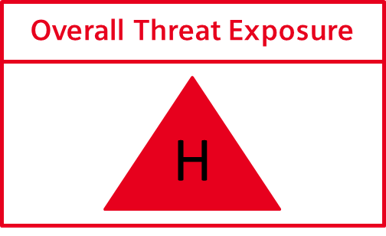
\includegraphics{Images/HighThreat.png}} 
% 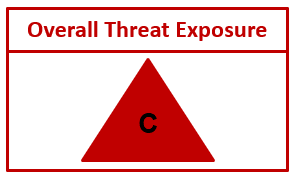
\includegraphics{Images/CriticalThreat.png}, 
% 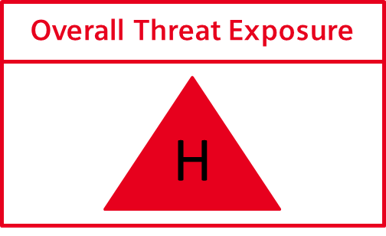
\includegraphics{Images/HighThreat.png}, 
% \includegraphics{Images/MediumThreat.png}, 
% 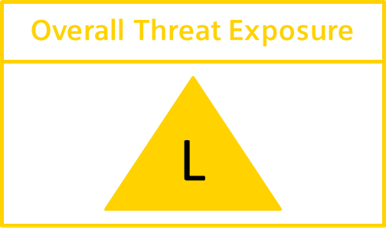
\includegraphics{Images/LowThreat.png}

\newcommand{\FindingsCountCritical}{0}
\newcommand{\FindingsCountHigh}{1}
\newcommand{\FindingsCountMedium}{2}
\newcommand{\FindingsCountLow}{2}
\newcommand{\FindingsCountInfo}{2}
\newcommand{\FindingsCountTotal}{7}
%----------------------------------------------------------------------------------------
%	DOCUMENT TYPE
%----------------------------------------------------------------------------------------

% Use "\ReportDocument" & "\TitlePageTableReport" when writing Report 
% Use "\ScopeDocument" & "\TitlePageTableScope" for creating Scope Document
\newcommand{\DocumentType}{\ReportDocument}
\renewcommand{\SetTitlePageTable}{\TitlePageTableReport}

%----------------------------------------------------------------------------------------
%	TITLE PAGE
%----------------------------------------------------------------------------------------
\newcommand{\ReportProjectName}{\xspace}
\newcommand{\ReportProjectType}{\xspace}
\newcommand{\AssetType}{\xspace}

%----------------------------------------------------------------------------------------
%	AUTHORS, REVIEWERS, APPROVERS
%----------------------------------------------------------------------------------------
\newcommand{\ReportDocumentMainAuthor}{Lukas Nad}
\newcommand{\ReportDocumentAuthor}{Lukas Nad}
\newcommand{\ReportDocumentReviewer}{}
\newcommand{\ReportDocumentApprover}{Filip Mrocek}

%----------------------------------------------------------------------------------------
%	DOCUMENT VERSION HISTORY
%----------------------------------------------------------------------------------------
% Document version history. Copy the inner line for subsequent version entries.
% Example: \ReportVersionEntry{DATE}{VERSION}{FIRSTNAME LASTNAME}{draft / review / released}{COMMENT}

% TODO: investigate git version tags (automatic compilation of document history table)

\newcommand{\ReportDocumentHistory}{
}


%----------------------------------------------------------------------------------------
%	GENERAL DOCUMENT INFORMATION
%----------------------------------------------------------------------------------------
\newcommand{\FiscalYear}{}
\newcommand{\ReportVersion}{Default}
\newcommand{\ReportDate}{June 12, 2023}
\newcommand{\ReportDocumentClassification}{CONFIDENTIAL}

\newcommand{\ReportStatus}{} 
% \newcommand{\ReportStatus}{DRAFT} 
%----------------------------------------------------------------------------------------
%	IN SCOPE
%----------------------------------------------------------------------------------------
\newcommand{\InScope}{

	\hline
	APK file & Android application  \\
	IPA file & iOS application \\
	Source code & Static analysis \\						
}


%----------------------------------------------------------------------------------------
%	WORST CASE SCENARIOS
%----------------------------------------------------------------------------------------

% Not needed for Scope Document
% Required for Report


\newcommand{\WorstCaseScenariosReport}{

\begin{xltabular}{\textwidth}{|l|X|c|c|c|c|c|c|c|}
	\hline 
	\cellcolor{grey230}  \textbf{Finding \#} &	 \cellcolor{grey230} \textbf{Description} & \cellcolor{grey230}
	
	\textbf{WS1} & \cellcolor{grey230} \textbf{WS2} & \cellcolor{grey230} \textbf{WS3} & \cellcolor{grey230} \textbf{WS4}\\
    \hline 
	1		&	ePHI is stored on device without encryption   & \Huge $\cdotp$ & \Huge $\cdotp$ & \Huge \phantom{} & \Huge \phantom{} \\
	\hline
	2		&	Sensitive Information Disclosure via Logging   & \Huge $\cdotp$ & \Huge $\cdotp$ & \Huge $\cdotp$  & \Huge \phantom{} \\
	\hline
	3		&	Weak Application Signature   & \Huge \phantom{} & \Huge \phantom{} & \Huge $\cdotp$  & \Huge $\cdotp$ \\
	\hline
	4		&	Heap Inspection of Sensitive Memory   & \Huge $\cdotp$ & \Huge $\cdotp$ & \Huge $\cdotp$  & \Huge \phantom{} \\
	\hline
	5		&	Outdated Components   & \Huge \phantom{} & \Huge \phantom{} & \Huge \phantom{}  & \Huge \phantom{} \\
	\hline
	6		&	DummyApplication Signed with a Debug Certificate   & \Huge \phantom{} & \Huge \phantom{} & \Huge \phantom{} & \Huge \phantom{} \\
	\hline
	7		&	Missing Enforced Updating   & \Huge \phantom{} & \Huge \phantom{} & \Huge \phantom{} & \Huge \phantom{} \\
	\hline
	
	\caption{Findings case scenarios} \label{table:FindingCaseScenarios}
\end{xltabular}
}


% Required for Scope & Report.
\newcommand{\WorstCaseScenariosScope}{
	\hline
	WS1	&	Information leakage of personal /patient data/customer data	\\
	WS2	&	Modification or corruption of data	\\
	WS3	&	Unauthorized read/write access to application/database	\\
	WS4	&	Asset becomes partly or completely unavailable	\\
}



%----------------------------------------------------------------------------------------
%	OUT OF SCOPE
%----------------------------------------------------------------------------------------
\newcommand{\OutOfScope}{
    \hline
	3rd party plugins	&  	 Plugins not developed by Siemens	\\		
	Underlying operating systems	& 	Android and iOS	\\
	REST APIs 	& Was already tested \\ 
}

%----------------------------------------------------------------------------------------
%	ENVIRONMENT
%----------------------------------------------------------------------------------------
\newcommand{\Environment}{
    
    \ReportAssessmentTeamLong obtained following access methods to DummyApplication: 
	\begin{itemize}
		\item Android APK file,
		\item iOS IPA file,
		\item application source code,
		\item test user credentials.
	\end{itemize}
}

%----------------------------------------------------------------------------------------
%	TEST PROTOCOL: TARGET
%----------------------------------------------------------------------------------------
\newcommand{\TargetTestProtocol}{https://TODOTODO}

%
%		File:		Testing_Methodology.tex
%		Author: 	Dusan Repel (SHS TE DC CYS CSA)
%		Date:		02/09/2020
%
%
\clearpage

\chapter{Testing Methodology}
\label{chapter:TestingMethodology}


%----------------------------------------------------------------------------------------
%	TOOLS USED
%----------------------------------------------------------------------------------------
\section{Tools Used}
\label{section:ToolsUsed}

During the course of the penetration test, the following tools were utilized:

\begin{xltabular}{\textwidth}{|l|l|l|X|}
	\hline
	\cellcolor{grey230}\textbf{Tool} & \cellcolor{grey230}\textbf{Version} & \cellcolor{grey230}\textbf{Test Type} & \cellcolor{grey230}\textbf{Work Type}\\
	\ToolsUsed
	
%	Tenable Nessus 8.2.3 Automatic scan
%Manual verification
%Port and vulnerability
%scanning
%Burp Suite Professional 2.1.04 Manual testing HTTP Traffic inspection and
%manipulation
%OWASP ZAP 2.8.1 Manual testing HTTP Traffic inspection and
%manipulation
%Nmap 7.80 Automatic scan Port enumeration and
%information gathering
%JAD v1.5.8g Manual
%decompilation
%Java bytecode decompilation
%JD-GUI v1.6.6 Automated
%decompilation
%Java package unpacking and
%bytecode decompilation
%dnSpy v6.1.4 Manual verification .NET decompilation and
%debugging
%Checkmarx v8.9.0 Automated scan Static analysis of Java
%decompilations
%x64dbg (Apr 29 2020
%build)
%Manual verification Debugging of x64 compiled
%machine code
%Immunity debugger v1.85 Manual verification Debugging of x86 compiled
%machine code
%PE Explorer v1.99 R6 Manual verification Disassembling of x86 PE
%executables
%CFF Explorer VIII Manual verification Parsing of PE executable
%headers
%JavaSnoop v1.0, v1.0 RC4,
%v1.1 RC2
%Manual verification Runtime instrumentation of
%Java bytecode
%Sysinternal Process Monitor v3.53 Manual verification Windows API hooking of
%target process to inspect calls
%Java JDK v1.6, v1.8, v14.0.1 Java environment Java compilation software
%Java JRE v1.6, v1.8 Java environment Java virtual machine
%FindBugs v3.0.1 Manual verification Static analysis on Java
%packages
%Process Explorer v16.32 Manual verification Inspection of Windows
%processes
%NetBeans v11.3 Manual compilation Compilation of Java source
%code decompilations
\caption{Tools employed} \label{table:ToolsEmployed}
\end{xltabular}



%----------------------------------------------------------------------------------------
%	ATTACK VECTORS AND PAYLOAD TYPES
%----------------------------------------------------------------------------------------
\section{Attack Vectors and Payload Types}
\label{section:AttackVectorsPayloadTypes}
\AttackVectors




%% Pentest Team Members
%\newcommand{\MiroH}{Miroslav Hricko & \PTORGSDS & miroslav.hricko@siemens-healthineers.com}
%\newcommand{\ViktorK}{Viktor Kristofiak & \PTORGCSA & viktor.kristofiak@siemens-healthineers.com}
%\newcommand{\NickY}{Mykola Yanko & \PTORGCSA & mykola.yanko@siemens-healthineers.com}
%\newcommand{\LukasN}{Lukas Nad & \PTORGCSA & lukas.nad@siemens-healthineers.com}
%\newcommand{\DusanR}{Dusan Repel & \PTORGSDS & dusan.repel@siemens-healthineers.com}
%\newcommand{\MiroK}{Miroslav Kuco & \PTORGCSA & miroslav.kuco@siemens-healthineers.com}
%\newcommand{\AndrejH}{Andrej Hlubik & \PTORGCSA & andrej.hlubik@siemens-healthineers.com}

\newcommand{\MiroH}{Miroslav Hricko & \PTORGSDS & \href{mailto://miroslav.hricko@siemens-healthineers.com}{miroslav.hricko\footnotemark[1]}}

\newcommand{\ViktorK}{Viktor Kristofiak & \PTORGCSA & \href{mailto://viktor.kristofiak@siemens-healthineers.com}{viktor.kristofiak\footnotemark[1]}}
\newcommand{\NickY}{Mykola Yanko & \PTORGCSA & \href{mailto://mykola.yanko@siemens-healthineers.com}{mykola.yanko\footnotemark[1]}}
\newcommand{\LukasN}{Lukas Nad & \PTORGCSA & \href{mailto://lukas.nad@siemens-healthineers.com}{lukas.nad\footnotemark[1]}}
\newcommand{\MiroK}{Miroslav Kuco & \PTORGCSA & \href{mailto://miroslav.kuco@siemens-healthineers.com}{miroslav.kuco\footnotemark[1]}}
\newcommand{\AndrejH}{Andrej Hlubik & \PTORGCSA & \href{mailto://andrej.hlubik@siemens-healthineers.com}{andrej.hlubik\footnotemark[1]}}
\newcommand{\KatkaA}{Katarina Amrichova & \PTORGCSA & \href{mailto://katarina.amrichova@siemens-healthineers.com}{katarina.amrichova\footnotemark[1]}}
\newcommand{\PeterK}{Peter Kytka & \PTORGCSA & \href{mailto://peter.kytka@siemens-healthineers.com}{peter.kytka\footnotemark[1]}}
\newcommand{\EnzoP}{Enzo Massimiliano Pasquale & \PTORGCSA & \href{mailto://enzo-massimiliano.pasquale@siemens-healthineers.com}{enzo-massimiliano.pasquale\footnotemark[1]}}
\newcommand{\JozefS}{Jozef Frantisek Stefanovic & \PTORGCSA & \href{mailto://jozef-frantisek.stefanovic@siemens-healthineers.com}{jozef-frantisek.stefanovic\footnotemark[1]}}
\newcommand{\JanS}{Jan Svitic & \PTORGCSA & \href{mailto://jan.svitic@siemens-healthineers.com}{jan.svitic\footnotemark[1]}}
\newcommand{\MichalO}{Michal Olencin & \PTORGCSA & \href{mailto://michal.olencin@siemens-healthineers.com}{michal.olencin\footnotemark[1]}}

\newcommand{\ChaitanyaBM}{Chaitanya B.M & \PTORGCYSLAB & \href{mailto://chaitanya@siemens-healthineers.com}{chaitanya\footnotemark[1]}}
\newcommand{\SreenithaN}{Sreenitha N. & \PTORGCYSLAB & \href{mailto://sreenitha.n@siemens-healthineers.com}{sreenitha.n\footnotemark[1]}}
\newcommand{\SaurabhP}{Saurabh Prasad & \PTORGCYSLAB & \href{mailto://saurabh.prasad@siemens-healthineers.com}{saurabh.prasad\footnotemark[1]}}
\newcommand{\ShivamY}{Shivam Yadav & \PTORGCYSLAB & \href{mailto://shivam.yadav@siemens-healthineers.com}{shivam.yadav\footnotemark[1]}}
\newcommand{\TakshM}{Medhavi Taksh & \PTORGCYSLAB & \href{mailto://taksh.bhatt@siemens-healthineers.com}{taksh.bhatt\footnotemark[1]}}

\newcommand{\AnkitCh}{Ankit Chandgadkar & \PTORGCHMPE & \href{mailto://ankit.chandgadkar@varian.com}{ankit.chandgadkar\footnotemark[2]}}
\newcommand{\JayK}{Jay Kapadiya & \PTORGCHMPE & \href{mailto://jay.kapadiya@varian.com}{jay.kapadiya\footnotemark[2]}}

\newcommand{\newmember}{NewMember & \NewMemberDep & \href{mailto://newmember@siemens-healthineers.com}{newmember\footnotemark[\value{footnote}]}}

%\newcommand{\MiroH}{Miroslav Hricko & \PTORGSDS & miroslav.hricko\footnotemark[\value{footnote}]}
%\newcommand{\ViktorK}{Viktor Kristofiak & \PTORGCSA & viktor.kristofiak\footnotemark[\value{footnote}]}
%\newcommand{\NickY}{Mykola Yanko & \PTORGCSA & mykola.yanko\footnotemark[\value{footnote}]}
%\newcommand{\LukasN}{Lukas Nad & \PTORGCSA & lukas.nad\footnotemark[\value{footnote}]}
%\newcommand{\DusanR}{Dusan Repel & \PTORGSDS & dusan.repel\footnotemark[\value{footnote}]}
%\newcommand{\MiroK}{Miroslav Kuco & \PTORGCSA & miroslav.kuco\footnotemark[\value{footnote}]}
%\newcommand{\AndrejH}{Andrej Hlubik & \PTORGCSA & andrej.hlubik\footnotemark[\value{footnote}]}

%% Pentest ORG Codes
%\newcommand{\PTORGCSA}{SHS TE DC CYS CSA}
%\newcommand{\PTORGSDS}{SHS TE DC CYS CSA SDS}
\newcommand{\PTORGGDC}{SHS TE DC IND ST}
\newcommand{\PTORGCYSLAB}{SHS TE DC CYS LAB}
\newcommand{\PTORGCHMPE}{SHS TE CYS CHM PE}

\newcommand{\PTORGCSA}{SHS TE DC CYS CSA P\&PA}
\newcommand{\PTORGSDS}{SHS TE DC CYS CSA}


\newcommand{\NewMemberDep}{Member Department}
%----------------------------------------------------------------------------------------
%	SCOPE: PARTICIPANTS AND CONTACTS
%----------------------------------------------------------------------------------------

% Set table "Participants and Contacts": Scope table or Report table
\newcommand{\SetParticipantsAndContactsTable}{\ReportParticipantsAndContacts}

% Report Table
\newcommand{\ReportParticipantsAndContacts}{
    \begin{xltabular}{\textwidth}{|X|X|X|X|}
        \hline
        \cellcolor{grey230}\textbf{Role} & \cellcolor{grey230}\textbf{Name} & \cellcolor{grey230}\textbf{Department} & \cellcolor{grey230}\textbf{Contact} \\
    
        \hline
        Application Manager & \ApplicationManager & \ApplicationManagerDepartment & \ApplicationManagerContact \\
    
        %\hline
        %Business Owner & \BusinessOwnerName & \BusinessOwnerDepartment & \BusinessOwnerContact \\
    
        %\hline
        %Business Representative & \BusinessRepresentativeName & \BusinessRepresentativeDepartment & \BusinessRepresentativeContact\\
    
        \hline
        \multirow[t]{\TechnicalContactsNumber}{*}{Technical Contacts} & \TechnicalContacts
        \hline
        Pentest Coordinator & \PentestCoordinatorName & \PentestCoordinatorDepartment &  \PentestCoordinatorContact \\ 
    
        \hline
        Pentest Project Lead & \PentestLeadName	&  \PentestLeadDepartment &  \PentestLeadContact \\ 
    
        \hline
        \multirow[t]{\PentestParticipantsNumber}{*}{Pentest Team} & \PentestTeamMember
        \hline
    
    \caption{Test participants and contacts} \label{table:TestParticipantsContacts}
    \end{xltabular}
}

% Scope Table
\newcommand{\ScopeParticipantsAndContacts}{
    \begin{xltabular}{\textwidth}{|l|X|X|X|}
        \hline
        \cellcolor{grey230}\textbf{Role} & \cellcolor{grey230}\textbf{Name} & \cellcolor{grey230}\textbf{Department} & \cellcolor{grey230}\textbf{Contact} \\
    
        \hline
        Application Manager & \ApplicationManager & \ApplicationManagerDepartment & \ApplicationManagerContact \\
    
        \hline
        Business Owner & \BusinessOwnerName & \BusinessOwnerDepartment & \BusinessOwnerContact \\
    
        \hline
        Business Representative & \BusinessRepresentativeName & \BusinessRepresentativeDepartment & \BusinessRepresentativeContact\\
    
        \hline
        \multirow[t]{\TechnicalContactsNumber}{*}{Technical Contacts} & \TechnicalContacts
        \hline
        Pentest Coordinator & \PentestCoordinatorName & \PentestCoordinatorDepartment & \PentestCoordinatorContact \\ 
        \hline
    \caption{Test participants and contacts} \label{table:TestParticipantsContacts}
    \end{xltabular}
}
\input{./Static/Scope_Document/General_Scope.tex}
%----------------------------------------------------------------------------------------
%	SCOPE: TARGET INFORMATION
%----------------------------------------------------------------------------------------

% Set target text in "Target Information": Scope text or Report text
\newcommand{\SetTargetInformation}{\ReportTargetInformation}

\newcommand{\ReportTargetInformation}{
    In agreement with the \textbf{Application Manager}, the Penetration Test has been conducted on the following target:
}
\newcommand{\ScopeTargetInformation}{
    In agreement with the \textbf{Application Manager}, the Penetration Test will be conducted on the following target:
}

%----------------------------------------------------------------------------------------
%	SCOPE: TEST LOCATION AND DURATION
%----------------------------------------------------------------------------------------

% Set target text in "Test Location and Duration": Scope text or Report text
\newcommand{\SetLocationAndDuration}{\ReportLocationAndDuration}

\newcommand{\ReportLocationAndDuration}{
    The Penetration test was performed remotely and on site from Siemens Healthineers Bratislava, Kosice and Zilina (Slovakia).
}

\newcommand{\ScopeLocationAndDuration}{
    The Penetration test will be performed remotely from Siemens Healthineers Bratislava (Slovakia).
}
%----------------------------------------------------------------------------------------
%	SCOPE: SCOPE AND PROCEDURES
%----------------------------------------------------------------------------------------

% Set section "Participants and Contacts": Scope or Report section
\newcommand{\SetScopeAndProceduresSection}{\ReportScopeAndProceduresSection}








% Report Section
\newcommand{\ReportScopeAndProceduresSection}{

%----------------------------------------------------------------------------------------
%	IN SCOPE
%----------------------------------------------------------------------------------------
\chapter{Scope and Procedures}
\label{chapter:ScopeAndProcedures}

\section{Scope}
\label{section:Scope}

In alignment with the Application Manager, the following components of \textbf{\TargetInfoName} have been tested during this assessment:

\begin{xltabular}{\textwidth}{|l|X|}
	\hline
	\cellcolor{grey230} \textbf{Components} & \cellcolor{grey230} \textbf{Details}  \\
	\InScope
	\hline
	\caption{Scope} \label{table:Scope}
\end{xltabular}


%----------------------------------------------------------------------------------------
%	WORST CASE SCENARIOS
%----------------------------------------------------------------------------------------
\section{Worst Case Scenarios}
\label{section:WorstCaseScenarios}

Below is a list of worst-case scenarios defined together with the \textbf{Application Manager}.

\begin{xltabular}{\textwidth}{|l|X|}
	\hline
	\cellcolor{grey230} \textbf{\#} & \cellcolor{grey230} \textbf{Worst-case scenario}  \\
	\WorstCaseScenariosScope
	\hline
	\caption{Worst-case scenarios} \label{table:WorstCaseScenarios}
\end{xltabular}

\clearpage
The following table contains all worst-case scenarios and findings and if they could be realized within the Penetration test:
\WorstCaseScenariosReport


%----------------------------------------------------------------------------------------
%	OUT OF SCOPE
%----------------------------------------------------------------------------------------
\clearpage
\section{Out Of Scope}
\label{section:OutOfScope}

In alignment with the Application Manager, the following components of \textbf{\TargetInfoName} were not tested during this assessment:

\begin{xltabular}{\textwidth}{|l|X|}
	\hline
	\cellcolor{grey230} \textbf{Components} & \cellcolor{grey230} \textbf{Details}  \\
	\OutOfScope
	\hline
	\caption{Out Of Scope} \label{table:OutOfScope}
\end{xltabular}


%----------------------------------------------------------------------------------------
%	ENVIRONMENT
%----------------------------------------------------------------------------------------
\section{Environment}
\label{section:Environment}

\Environment
}









% Scope section
\newcommand{\ScopeDocScopeAndProceduresSection}{

%----------------------------------------------------------------------------------------
%	IN SCOPE
%----------------------------------------------------------------------------------------
\chapter{Scope and Procedures}
\label{chapter:ScopeAndProcedures}

\section{In Scope}
\label{section:InScope}

In alignment with the \textbf{Application Manager}, the following components of \textbf{\TargetInfoName} will be tested during this assessment:

\begin{xltabular}{\textwidth}{|l|X|}
	\hline
	\cellcolor{grey230} \textbf{Components} & \cellcolor{grey230} \textbf{Details}  \\
	\InScope
	\hline
	\caption{In Scope} \label{table:InScope}
\end{xltabular}


%----------------------------------------------------------------------------------------
%	WORST CASE SCENARIOS
%----------------------------------------------------------------------------------------
\section{Worst Case Scenarios}
\label{section:WorstCaseScenarios}

Below is a list of worst-case scenarios defined together with the \textbf{Application Manager} \& \textbf{Business Representative}.

\begin{xltabular}{\textwidth}{|l|X|}
	\hline
	\cellcolor{grey230} \textbf{\#} & \cellcolor{grey230} \textbf{Worst-case scenario}  \\
	\WorstCaseScenariosScope
	\hline
	\caption{Worst-case scenarios} \label{table:WorstCaseScenarios}
\end{xltabular}

%----------------------------------------------------------------------------------------
%	OUT OF SCOPE
%----------------------------------------------------------------------------------------
\section{Out Of Scope}
\label{section:OutOfScope}

In alignment with the Application Manager, the following components of \textbf{\TargetInfoName} will not tested during this assessment:

\begin{xltabular}{\textwidth}{|l|X|}
	\hline
	\cellcolor{grey230} \textbf{Components} & \cellcolor{grey230} \textbf{Details}  \\
	\OutOfScope
	\hline
	\caption{Out Of Scope} \label{table:OutOfScope}
\end{xltabular}

}

\newcommand{\FindingAuthor}{squarepants}
\newcommand{\FindingNumber}{0}
\newcommand{\FindingName}{x123}
\newcommand{\Criticality}{sponge}
\newcommand{\Exploitability}{x123}
\newcommand{\Category}{x123}
\newcommand{\Location}{x123}
\newcommand{\Detail}{x123}
\newcommand{\Component}{x123}
\newcommand{\Detectability}{x123}    	
\newcommand{\FoundWith}{x123}
\newcommand{\TestMethod}{x123}
\newcommand{\CVSS}{x123}
\newcommand{\CVSSvector}{x123}
\newcommand{\CWE}{x123}

%
%		File:		Header_Footer.tex
%		Author: 	Dusan Repel (SHS TE DC CYS CSA)
%		Date:		02/09/2020
%
%
% Graphics & figures 
\RequirePackage[pdftex]{graphicx} 
\DeclareGraphicsExtensions{.pdf,.PDF,.jpg,.JPG,.png,.PNG,}
\RequirePackage{tikz}
\RequirePackage{pdfpages}                                   % Inclusion of PDF pages in the appendix

% Language support
\RequirePackage[T1]{fontenc}
\RequirePackage[utf8]{inputenc}
\RequirePackage[english]{babel}

% Page manipulation
\RequirePackage[margin=2cm]{geometry}                       % Uses smaller margins for more text per page
\RequirePackage{lastpage}                                   % Gets the number of last page
\RequirePackage{fancyhdr}                                   % Enables headers and footers
\setcounter{tocdepth}{3}                                    % Set max. depth of TOC
\RequirePackage{currfile}                                   % Get the name of the currently included file

% Text manipulation
\RequirePackage{varioref}                                   % Enable reference with automatic concatenation of strings 
\RequirePackage{datetime}                                   % Enable date/time formating
\newdateformat{ReportYear}{\THEYEAR}
\RequirePackage[hyphens,spaces,obeyspaces]{url}             % Enable URL formatting
\def\UrlBreaks{\do\.\do\@\do\\\do\/\do\!\do\|\do\;\do\>\do\[\do\]\do\$\do\^\do\(\do\)\do\,\do\?\do\'\do+\do\#\do\a\do\b\do\c\do\d\do\e\do\f\do\g\do\h\do\i\do\j\do\k\do\l\do\m\do\n\do\o\do\p\do\q\do\r\do\s\do\t\do\u\do\v\do\w\do\x\do\y\do\z\do\A\do\B\do\C\do\D\do\E\do\F\do\G\do\H\do\I\do\J\do\K\do\L\do\M\do\N\do\O\do\P\do\Q\do\R\do\S\do\T\do\U\do\V\do\W\do\X\do\Y\do\Z\do\0\do\1\do\2\do\3\do\4\do\5\do\6\do\7\do\8\do\9\do\-\do\*\do\-\do\~\do\'\do\"\do\-\do\=\do\_\do\:\do\&\do\\\do\%\do\{\do\}}
\RequirePackage{rotating}                                   % Enables rotation of text
\RequirePackage{pslatex}                                    % Sets style of fonts: Roman=Times,Serif=Helvetica,Mono=Courier
\RequirePackage[]{titlesec}                                 % Enables manipulation of titles (chapter, section, etc)
\titleformat{\chapter}
{\normalfont\Huge\bfseries}
{\thechapter}{5mm}{}
\titlespacing{\chapter}
{0mm}{-5mm}{0mm}[0mm]
\RequirePackage{textcomp}                                   % For extended symbol support
\RequirePackage{amsfonts}                                   % Set default fonts
\renewcommand{\rmdefault}{phv}
\renewcommand{\sfdefault}{pti}
\RequirePackage{amssymb}                                    % math symbols
\RequirePackage{pifont}                                     % Enables dingbats
\RequirePackage{xspace}                                     % Enables dynamic placement of spaces, e.g. when defining custom macros 

% Object manipulation
\RequirePackage{float}                                      % Allows mandatory positioning of floats (figures, tables, ...)
\RequirePackage{placeins}                                   % Prevents objects from floating into following sections
\RequirePackage{fancyvrb}                                   % Enables the inclusion of verbatim environments in tables

% Table manipulation
\RequirePackage{multirow}                                   % Enables the aggregation of multiple rows
\RequirePackage{multicol}                                   % Enables the aggregation of multiple columns
\RequirePackage{colortbl}                                   % Enables colors in tables
\RequirePackage{tabularx}                                   % Enhances table support
\RequirePackage{longtable}                                  % Enables tables to exceed one page
\RequirePackage{diagbox}                                    % Enables diagonally split cells in tables
\RequirePackage{hhline}                                     % Enables pretty double lines 

% Listings
\RequirePackage{listings}
\lstset{
	basicstyle=\footnotesize\ttfamily, 
	numbers=left,               
	numberstyle=\footnotesize,
	numbersep=7pt,              
	tabsize=2,                  
	extendedchars=true,         
	breaklines=true,            
	frame=tb,  
	captionpos=b       
	showspaces=false,           
	showtabs=false,     
	xleftmargin=20pt,
	framexleftmargin=15pt,
	framexrightmargin=-5pt,
	framexbottommargin=2pt,
	framextopmargin=2pt,
	showstringspaces=false,
	aboveskip=20pt
}

% Enumerate and Itemize
\RequirePackage{enumitem}                                   % Enables customized setting of distances around enumerate and itemize

\RequirePackage{framed} 
\RequirePackage{xcolor} 
\colorlet{shadecolor}{gray!25} 

% Must be last package included
\RequirePackage[pdftex,colorlinks=false,breaklinks=true,pdfborder={0 0 0}]{hyperref}


\newcounter{ReportCounterFinding}
\setcounter{ReportCounterFinding}{0} 
\newcounter{ReportCounterAppendix}
\setcounter{ReportCounterAppendix}{0} 

% Symbol definition
\newcommand{\xmark}{\ding{55}}                              % Defines checkmark

% Color definitions
% SHS Colors
\definecolor{orangeshs236}{RGB}{236,102,2}
\definecolor{orangeshs242}{RGB}{242,146,87}
\definecolor{petrolshs122}{RGB}{122,22,45}
\definecolor{petrolshs168}{RGB}{168,108,115}
\definecolor{petrolsag}{RGB}{0,153,153}
\definecolor{yellowshs}{RGB}{255,210,0}
\definecolor{redshs}{RGB}{231,0,29}
\definecolor{greenshs}{RGB}{0,154,56}
\definecolor{grey64}{RGB}{0.64,0.64,0.64}
\definecolor{grey128}{RGB}{128,128,128}
\definecolor{grey191}{RGB}{0.191,0.191,0.191}
\definecolor{grey230}{RGB}{230,230,230}
\definecolor{blackshs}{RGB}{0,0,0}

%SAG Colors
\definecolor{siemenspetrol}{cmyk}{1.0,0.0,0.4,0.0}
\definecolor{healthineerspetrol}{cmyk}{0.744,0.000,0.329,0.188} % RGB #35CF8B
\definecolor{healthineersorange}{cmyk}{0.000,0.694,0.400,0.000} % RGB #FF4E00
\definecolor{ctlightgray}{cmyk}{0.0,0.0,0.0,0.13}
\definecolor{ctdarkgray}{cmyk}{0.0,0.0,0.0,0.35}
\definecolor{ctred}{cmyk}{0.0,1.0,1.0,0.05}
\definecolor{ctgreen}{cmyk}{1.0,0.0,1.0,0.0}
\definecolor{Critical}{RGB}{192,0,0}
\definecolor{High}{cmyk}{0.0,1.0,1.0,0.05}
\definecolor{High+Compliance}{cmyk}{0.0,1.0,1.0,0.05}
\definecolor{Medium}{cmyk}{0.0,0.6,1.0,0.0}
\definecolor{Medium+Compliance}{cmyk}{0.0,0.6,1.0,0.0}
\definecolor{Moderate}{cmyk}{0.0,0.6,1.0,0.0}
\definecolor{Moderate+Compliance}{cmyk}{0.0,0.6,1.0,0.0}
\definecolor{Low}{cmyk}{0.0,0.1,1.0,0.0}
\definecolor{Low+Compliance}{cmyk}{0.0,0.1,1.0,0.0}
\definecolor{Info}{cmyk}{0.0,0.0,0.0,0.35}
\definecolor{Info+Compliance}{cmyk}{0.0,0.0,0.0,0.35}
\definecolor{Pass}{cmyk}{0.92,0,0.87,0.09}
\definecolor{Compliance}{cmyk}{0.85,0.45,0.0,0.0}
\definecolor{CustomStatus}{cmyk}{1.0,1.0,1.0,1.0}

%
%	Added color definitions by dr
%
%\definecolor{Difficult}{cmyk}{0.0,1.0,1.0,0.05}
\definecolor{Difficult}{RGB}{231,0,29}

%\definecolor{Average}{cmyk}{0.0,0.6,1.0,0.0}
\definecolor{Average}{RGB}{242,146,87}

%\definecolor{Easy}{cmyk}{0.0,0.1,1.0,0.0}
\definecolor{Easy}{RGB}{255,210,0}

% \definecolor{TBR}{cmyk}{1.0,1.0,0.0,0.0}
\definecolor{TBR}{RGB}{0,0,255}

% Command used for cover pages
\newcommand{\ReportCoverPage}[4]{
	\par\noindent
	\vbox to 0.8\vsize{
		\hsize=0.1\hsize
		\vspace{1.0\vsize}
		\hbox to \hsize{\hfill#1\hfill}
	}
	\vbox to 0.8\vsize{
		\hsize=0.9\hsize
		\hbox{
			\vbox to 0.35\vsize{\par\noindent#2\vfill}
		}
		\hbox{
			\vbox to 0.55\vsize{\par\noindent#3\vfill}
		}
		\hbox{
			\vbox to 0.1\vsize{\par\noindent#4\vfill}
		}
	}
}

% Command for resolving a criticality level to a textual representation
\newcommand{\ReportResolveCriticalityText}[1]{%
\ifthenelse{\equal{#1}{High}}{High}{}%
\ifthenelse{\equal{#1}{High+Compliance}}{High (+Compliance)}{}%
\ifthenelse{\equal{#1}{Medium}}{Medium}{}%
\ifthenelse{\equal{#1}{Medium+Compliance}}{Medium (+Compliance)}{}%
\ifthenelse{\equal{#1}{Moderate}}{Moderate}{}%
\ifthenelse{\equal{#1}{Moderate+Compliance}}{Moderate (+Compliance)}{}%
\ifthenelse{\equal{#1}{Low}}{Low}{}%
\ifthenelse{\equal{#1}{Low+Compliance}}{Low (+Compliance)}{}%
\ifthenelse{\equal{#1}{Info}}{Info}{}%
\ifthenelse{\equal{#1}{Info+Compliance}}{Info (+Compliance)}{}%
\ifthenelse{\equal{#1}{Compliance}}{Compliance}{}%
\ifthenelse{\equal{#1}{Pass}}{Pass}{}%
\ifthenelse{\equal{#1}{TBR}}{TBR}{}%
}

% Command for Finding sections
\newcommand{\ReportFindingSection}[1]{	
	\renewcommand{\ReportBoolIsFirstFindingInSection}{true}
	\renewcommand{\ReportBoolUsesFindingSections}{true}
	\ifthenelse{\equal{\ReportBoolWriteSummary}{false}}{
		\ifthenelse{\equal{\theReportCounterFinding}{0}}{}{
			\FloatBarrier 
			\clearpage
		}
		\immediate\write\outfileSummary{\noexpand\ReportFindingSection{\unexpanded{#1}}}
	}{}
	\section{#1}
}

% Command for Finding header

\providecommand{\ReportCounterFindingautorefname}{Finding}
\newcommand{\ReportFindingHeader}[1] {
	

	\ifthenelse{\equal{\ReportBoolWriteSummary}{false}}{
		% 
		% Lukas
		% conditionally inserting clear pages
		% 
		\ifthenelse {\equal{\ReportBoolIsFirstFindingInSection}{true}}{}{\clearpage}
		
		\renewcommand{\ReportFindingFileName}{\FindingName} % double check, was #1
		\ifthenelse{\equal{\ReportBoolIsFirstFindingInSection}{false}}{\FloatBarrier}{}
		\refstepcounter{ReportCounterFinding}
		\label{\FindingName} % double check, was #1
		\ifthenelse{\equal{\ReportBoolUsesFindingSections}{true}}{
			\addcontentsline{toc}{subsection}{Finding \theReportCounterFinding: \FindingName} % double check, was #1
		}{
			\addcontentsline{toc}{section}{Finding \theReportCounterFinding: \FindingName} % double check, was #1
		}				
	}{
		\ifthenelse{\equal{\ReportBoolIsFirstFindingInSection}{true}}{}{\vspace{11mm}}
	}
	
	% Set Finding color boxes depending on the Finding status 
	\renewcommand{\ReportFindingColor}{\Criticality}
	
	\renewcommand{\arraystretch}{1.5}

	
	\ifthenelse{\equal{\ReportBoolWriteSummary}{false}} {
		\begin{tabularx}{\textwidth}{ m{0.7cm}|ll@{\hskip 1in}lX| }
		
				\multirow{8}{*}
				% {\cellcolor{\ReportFindingColor}} & \multicolumn{4}{l}{\cellcolor{grey-shs-217}\textbf{\textcolor{black}}{\Large\textbf{Finding \FindingNumber: \FindingName}}}\\
		
				{\cellcolor{\ReportFindingColor}} & \cellcolor{grey-shs-217}\textbf{\textcolor{black}}{\Large\textbf{Finding \FindingNumber:}} & \multicolumn{3}{p{12.42cm}}{\cellcolor{grey-shs-217}\textbf{\textcolor{black}}{\Large\textbf{\FindingName}}}\\
				
				\cellcolor{\ReportFindingColor} & \multicolumn{4}{r}{\cellcolor{grey-shs-217}\textbf{\textcolor{black}}{\small\textit{ID: \ReportProjectID}}}\\
				
				\cellcolor{\ReportFindingColor} & \textbf{Criticality:}    & \textcolor{\ReportFindingColor}{\textbf{\MakeUppercase{\Criticality}}}	& \textbf{Category:}  &  \Category \\ 
			
				\cellcolor{\ReportFindingColor} & \textbf{Detectability:}  &  \Detectability  &	\textbf{Exploitability:} &  \Exploitability\\
				
				\cellcolor{\ReportFindingColor} & \textbf{CWE / CVE:}  &  \href{https://cwe.mitre.org/data/definitions/\CWE.html}{CWE-\CWE}  & \textbf{CVSS Score:} &  \CVSS  \\
				\cellcolor{\ReportFindingColor} & \textbf{CVSS Vector:} & \multicolumn{3}{p{.7\textwidth}|}{\CVSSvector}\\
				
				\cellcolor{\ReportFindingColor} & \textbf{Location:} & \multicolumn{3}{p{.7\textwidth}|}{\Location}\\
				\cellcolor{\ReportFindingColor} & \textbf{Component:} & \multicolumn{3}{p{.7\textwidth}|}{\Component}\\
				
				\hline
			\end{tabularx}
		\vspace{0.5cm}
		
	}
	
	\ifthenelse{\equal{\ReportBoolWriteSummary}{true}} {
		\begin{tabularx}{\textwidth}{ m{0.7cm}|ll@{\hskip 1in}lX| }

			%\hline
		
			\multirow{8}{*}
			% {\cellcolor{\ReportFindingColor}} & \multicolumn{4}{l}{\cellcolor{grey-shs-217}\textbf{\textcolor{black}}{\Large\textbf{Finding \FindingNumber: \FindingName}}}\\
	
			{\cellcolor{\ReportFindingColor}} & \cellcolor{grey-shs-217}\textbf{\textcolor{black}}{\Large\textbf{Finding \FindingNumber:}} & \multicolumn{3}{p{12.42cm}}{\cellcolor{grey-shs-217}\textbf{\textcolor{black}}{\Large\textbf{\FindingName}}}\\
	
			\cellcolor{\ReportFindingColor} & \multicolumn{4}{r}{\cellcolor{grey-shs-217}\textbf{\textcolor{black}}{\small\textit{ID: \ReportProjectID}}}\\
			
			\cellcolor{\ReportFindingColor} & \textbf{Criticality:}    & \textcolor{\ReportFindingColor}{\textbf{\MakeUppercase{\Criticality}}}	& \textbf{Category:}  &  \Category\\ 
			
			\cellcolor{\ReportFindingColor} & \textbf{Detectability:}  &  \Detectability  &	\textbf{Exploitability:} &  \Exploitability\\
			
			\cellcolor{\ReportFindingColor} & \textbf{CWE / CVE:}  &  \href{https://cwe.mitre.org/data/definitions/\CWE.html}{CWE-\CWE}  & \textbf{CVSS Score:} &  \CVSS  \\
			\cellcolor{\ReportFindingColor} & \textbf{CVSS Vector:} & \multicolumn{3}{p{.7\textwidth}|}{\CVSSvector}\\
			
			\cellcolor{\ReportFindingColor} & \textbf{Location:} & \multicolumn{3}{p{.7\textwidth}|}{\Location}\\
			\cellcolor{\ReportFindingColor} & \textbf{Component:} & \multicolumn{3}{p{.7\textwidth}|}{\Component}\\
				
			\hline
			\cellcolor{\ReportFindingColor} & \multicolumn{4}{l|}{\textit{(Further details \vpageref{\FindingName}.)}}\\
			\hline 							
		
		\end{tabularx}
	}
	
	

	% \ifthenelse{\equal{\ReportBoolWriteSummary}{true}}
	% {
	% 	\textbf{Details:}
	% 	\FindingDetailsSummary
	% 	\textit{(Further details \vpageref{\FindingName}}
	% }
	
	%
	% Remove extra space in non-summary pages
	%
	\ifthenelse{\equal{\ReportBoolWriteSummary}{false}}
		{
			\vspace{-0.8cm}
		}{}
	
	%
	%	Write to outfile (Summary of Findings)
	%
	\ifthenelse{\equal{\ReportBoolWriteSummary}{false}} {
	
		\renewcommand{\FindingNumber}{\theReportCounterFinding}
		\immediate\write\outfileSummary{\noexpand\renewcommand{\noexpand\ReportFindingFileName}{\ReportFindingFileName}}
		
		\immediate\write\outfileSummary{\noexpand\renewcommand{\noexpand\FindingNumber}{\FindingNumber}}
		\immediate\write\outfileSummary{\noexpand\renewcommand{\noexpand\FindingName}{\FindingName}}
		\immediate\write\outfileSummary{\noexpand\renewcommand{\noexpand\Criticality}{\Criticality}}
		\immediate\write\outfileSummary{\noexpand\renewcommand{\noexpand\Detectability}{\Detectability}}
		\immediate\write\outfileSummary{\noexpand\renewcommand{\noexpand\Exploitability}{\Exploitability}}
		\immediate\write\outfileSummary{\noexpand\renewcommand{\noexpand\Category}{\Category}}
		\immediate\write\outfileSummary{\noexpand\renewcommand{\noexpand\Location}{\Location}}
		\immediate\write\outfileSummary{\noexpand\renewcommand{\noexpand\Component}{\Component}}
		%\immediate\write\outfileSummary{\noexpand\renewcommand{\noexpand\FindingDetailsSummary}{\FindingDetailsSummary}}
		\immediate\write\outfileSummary{\noexpand\renewcommand{\noexpand\CVSS}{\CVSS}}
		\immediate\write\outfileSummary{\noexpand\renewcommand{\noexpand\CVSSvector}{\CVSSvector}}
		\immediate\write\outfileSummary{\noexpand\renewcommand{\noexpand\CWE}{\CWE}}
		\immediate\write\outfileSummary{\noexpand\renewcommand{\noexpand\FoundWith}{\FoundWith}}
		\immediate\write\outfileSummary{\noexpand\renewcommand{\noexpand\TestMethod}{\TestMethod}}
		
		\immediate\write\outfileSummary{\noexpand\ReportFindingHeader{\unexpanded{\FindingName}}}
	}{}
	\renewcommand{\ReportBoolIsFirstFindingInSection}{false}

} %


% Command for figure
\newcommand{\ReportFigure}[3]{
	\begin{figure}[H]
		\begin{center}
			\includegraphics[width=#3\textwidth]{\ReportPathImages#1}
		\end{center}
		\vspace{-5mm} 
		\caption{#2}
		\label{#1}
	\end{figure}
}


% Command for note
\newcommand{\ReportNote}[1]{
	\paragraph{Note:}	#1
}

% Command for re-test
\newcommand{\ReTest}[1]{
	\paragraph{Re-Test:} #1
}

% Command for document version entry
\newcommand{\ReportVersionEntry}[4]{
	% \renewcommand{\ReportDate}{#1}
	\renewcommand{\ReportVersion}{#2}
	\ifthenelse{\equal{\ReportBoolWriteHistory}{true}}{#1 & #2 & #3 & #4 \\\hline}{}
}

% Definition of autoref names
\AtBeginDocument{%
	\renewcommand{\sectionautorefname}{Section}
	\renewcommand{\subsectionautorefname}{Section}
	\renewcommand{\subsubsectionautorefname}{Section}
	\renewcommand{\chapterautorefname}{Chapter}
	\renewcommand{\partautorefname}{Part}
	\renewcommand{\equationautorefname}{Equation}
	\renewcommand{\figureautorefname}{Figure}
	\providecommand{\subfigureautorefname}{}
	\renewcommand{\subfigureautorefname}{Figure}
	\renewcommand{\Itemautorefname}{Item}
	\renewcommand{\tableautorefname}{Table}
}

\newcommand{\enquote}[1]{``#1''}

%%%%%%%%%%%%%%%%%%%%%%%%%%%%%%%%%%%%%%%%%%%%%%%%%%%%%%%%%%%%%
%% Preamble
%%%%%%%%%%%%%%%%%%%%%%%%%%%%%%%%%%%%%%%%%%%%%%%%%%%%%%%%%%%%%


% Already parse document version information once for use on the first report pages
\renewcommand{\ReportBoolWriteHistory}{false}
\ReportDocumentHistory
\renewcommand{\ReportBoolWriteHistory}{true}


% Define document style 
\setlength{\topmargin}{-10mm}
\setlength{\headheight}{10mm}
\setlength{\textheight}{240mm}



\fancypagestyle{plain}{
	\lhead{\small \HeaderType \ReportProjectName \\ Version\ \ReportVersion ~- \ReportStatus}
	\chead{}
	%\rhead{\small \ReportAssessmentTeamLong~(\ReportAssessmentTeamShort) \\ X:\ \ReportDocumentClassification}
	\rhead{
\includegraphics[scale=0.2]{Images/shs-logo-4.png}}
	\renewcommand{\headrulewidth}{.5pt}
	%\lfoot{\small Project number:\ \ReportProjectNumber}
	
		% Footer
		%\color{gray}
		\lfoot{\small Classification: \ReportDocumentClassification}
		\cfoot{\small Page \thepage\ of \pageref*{LastPage}}  % Use pageref{LastPage} for hyperlink
		\rfoot{\small \monthdayyeardate\today}
	
	\renewcommand{\footrulewidth}{0.5pt}
}
\pagestyle{fancy}{
	\lhead{\small \HeaderType \ReportProjectName \\ Version\ \ReportVersion ~- \ReportStatus}
	\chead{}
	%\rhead{\small \ReportAssessmentTeamLong~(\ReportAssessmentTeamShort) \\ X:\ \ReportDocumentClassification}
	\rhead{
\includegraphics[scale=0.2]{Images/shs-logo-4.png}}
	
	\renewcommand{\headrulewidth}{.5pt}
	%\lfoot{\small Project number:\ \ReportProjectNumber}
	
	% Footer
	\lfoot{\small Classification: \ReportDocumentClassification}
	\cfoot{\small Page \thepage\ of \pageref*{LastPage}}
	\rfoot{\small \monthdayyeardate\today}
	\renewcommand{\footrulewidth}{0.5pt}
}

% Settings for reducing ocurrence of widows and orphans
\widowpenalty10000
\clubpenalty10000



\usepackage{keyval}
\usepackage{graphicx}
\usepackage{eso-pic}

\usepackage{tikz}
\usetikzlibrary{fit}

\usepackage[most]{tcolorbox}

\usepackage{lipsum}
\usepackage{afterpage}
\usepackage{overpic}
\usepackage{mdframed}
\usepackage{datetime}
\usepackage[capitalise]{cleveref}
\usepackage{pgf-pie}
\usepackage[misc]{ifsym}
\usepackage[utf8]{inputenc}
\usepackage[english]{babel}
\usepackage[numbers]{natbib}
\usepackage{url}
\usepackage{hyperref}
\usepackage{verbatim}
\usepackage{tabularx}
\usepackage{xcolor}
\usepackage{color, colortbl}
\usepackage{longtable}
\usepackage{xltabular}
\usepackage{array,booktabs,csvsimple}
\usepackage{subcaption}
\usepackage[export]{adjustbox}
\usepackage{listings}
\usepackage[titles]{tocloft}

%\usepackage{comment}
\usepackage{natbib}

% Inline citing of bibliography
%\usepackage{biblatex}
\usepackage{bibentry}

% Summaries
\usepackage{multicol}
\usepackage{adjmulticol}

\newlength{\mylength}
\settowidth{\mylength}{Short}
					

%\lstset{breaklines=true}

% Redefine how figures should be printed
\crefname{figure}{Figure}{Figure}

\hypersetup{
    colorlinks=true,
    linkcolor=blue,
    filecolor=magenta,      
    urlcolor=blue,
}

\newdateformat{monthdayyeardate}{%
  \monthname[\THEMONTH]~\THEDAY, \THEYEAR}
  
\newcommand{\printpercent}[2]{%
    \setcounter{z}{#1 / #2 * 100}
    $#1/#2*100=\arabic{z}\%$
}

% Define SHS Brand Colors
\definecolor{red-shs}{RGB}{231,0,29}
\definecolor{dark-red-shs}{RGB}{192,0,0}
\definecolor{orange-shs}{RGB}{236,102,2}
\definecolor{yellow-shs}{RGB}{255,210,0}
\definecolor{grey-shs}{RGB}{230,230,230}
\definecolor{grey-shs-217}{RGB}{217,217,217}
\definecolor{light-gray}{gray}{0.95}

% code
\newcommand{\code}[1]{\colorbox{light-gray}{\texttt{#1}}}


% Define the top table row color
\renewcommand{\arraystretch}{1.5}

% Table spaces between rows
\setlength{\extrarowheight}{1.5pt}

% Table top color
\arrayrulecolor{grey230}

%\usepackage{chronology}
\usepackage{chronosys}
  
\tikzset{flippedeventlabel/.append style={align=center}}

% Define PDF metadata
\hypersetup{
  pdftitle={\ReportProjectType~\ReportProjectName},
  pdfauthor={Siemens Healthineers \ReportAssessmentTeamLong},
  pdfsubject={\ReportProjectType~\ReportProjectName},
  pdfcreator={E55FEEBB350358369D62BA1274DE50BB6B8A1B11F0B1A7AF1202B6F419C9C99C},
  pdfkeywords={Siemens Healthineers \ReportProjectType~\ReportProjectName}
}

%----------------------------------------------------------------------------------------
%	WATERMARK SETUP
%----------------------------------------------------------------------------------------

\usepackage{background}
\ifthenelse{\equal{\ReportStatus}{RELEASE}}
{
    \backgroundsetup{contents=, opacity=0}
}
{
    \backgroundsetup{contents= DRAFT DRAFT,opacity=0.45}
}%


%----------------------------------------------------------------------------------------
%	BUILD SCOPE DOCUMENT
%----------------------------------------------------------------------------------------
\newcommand{\ScopeDocument}{
    \renewcommand{\SetParticipantsAndContactsTable}{\ScopeParticipantsAndContacts}
    \renewcommand{\HeaderType}{\HeaderScope}
    \renewcommand{\SetTargetInformation}{\ScopeTargetInformation}
    \renewcommand{\SetLocationAndDuration}{\ScopeLocationAndDuration}
    \renewcommand{\SetScopeAndProceduresSection}{\ScopeDocScopeAndProceduresSection}
    \renewcommand{\SetTitlePageTable}{\TitlePageTableScope}
\begin{document}
    
	%\nocite{*}
	%\bibliographystyle{plain}
	%\nobibliography{Bibliography}
	
    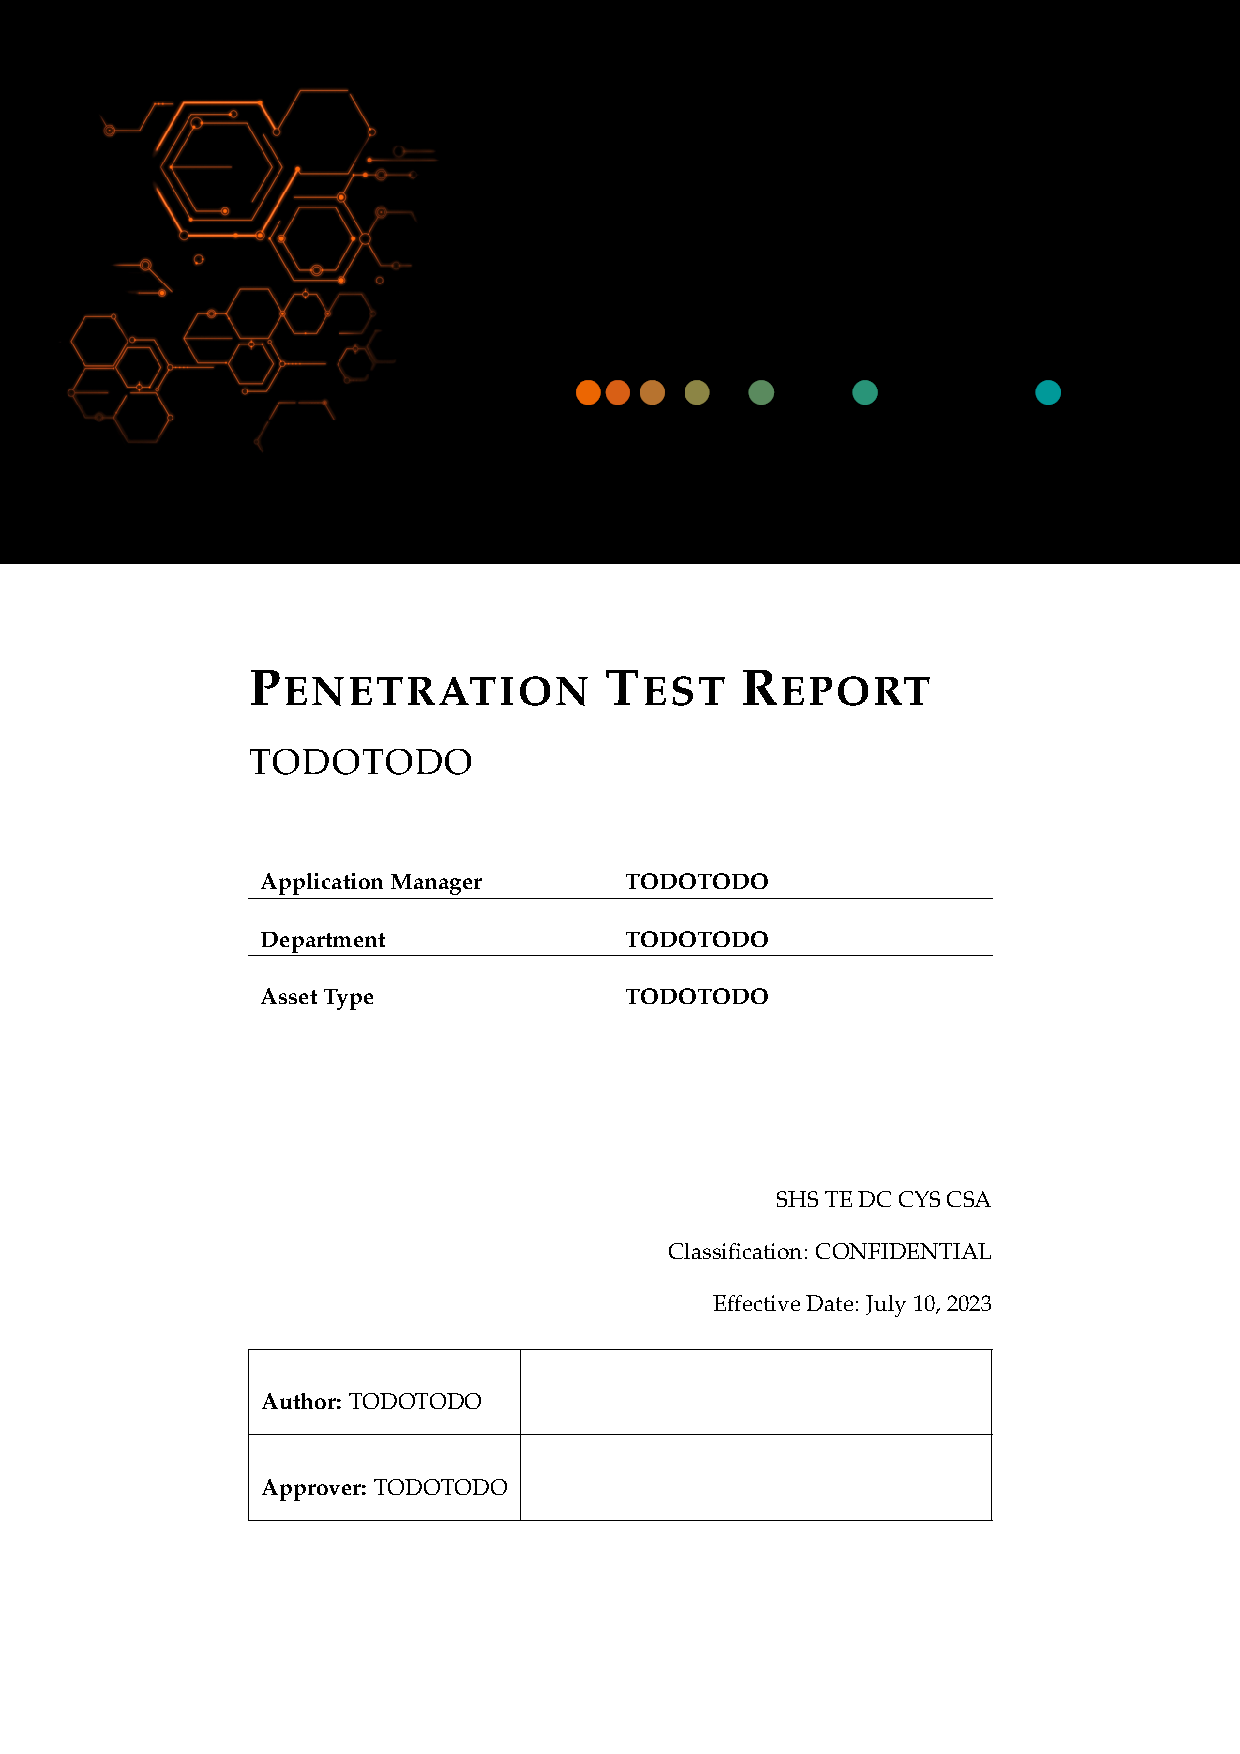
\includepdf{./TitlePage/TitlePage.pdf}
    \input{./Static/Scope_Document/General_Scope.tex}
    \chapter*{\color{orange-shs}Please carefully read the following points.}
\vskip 0.3in



\section*{Crucial Prerequisite}
\subsection*{Approval for third-party and SaaS applications}
For applications and systems, that are not hosted within Siemens Healthineers or in Azure/AWS Cloud, a written approval is required by the third party or SaaS vendor to conduct a penetration test.

\subsection*{Inform your provider/vendor}
Make sure the responsible operational staff is informed about the Penetration Test (e.g., ATOS, a SHS Datacenter, SHS Cloud Team and any third-party provider).

\subsection*{Review target information}
Review extensively the chapters In Scope and Out of scope, especially the details about your asset (e.g., URL’s, IP’s, Hostnames, etc.).



\section*{Rules of Engagement}
\subsection*{Target environment availability}
The Pentest Team requires access to the testing environment until the final report has been delivered.

\subsection*{Provision of partial pentest results}
No partial results will be provided unless a compelling reason requires it.

\subsection*{Configuration changes during testing}
Please avoid any configuration changes on the tested system during the penetration test, as this might have undesired effects on the pentest.



\vskip 0.3in
\begin{tcolorbox}[colback=red!5!white,colframe=red!75!black]
    \textbf{\large \underline{With the signature of this document}, the IT Application Manager confirms and agrees with the prerequisites and rules of engagement.}
  \end{tcolorbox}
    %----------------------------------------------------------------------------------------
%	DOCUMENT TYPE
%----------------------------------------------------------------------------------------

% Use "\ReportDocument" & "\TitlePageTableReport" when writing Report 
% Use "\ScopeDocument" & "\TitlePageTableScope" for creating Scope Document
\newcommand{\DocumentType}{\ReportDocument}
\renewcommand{\SetTitlePageTable}{\TitlePageTableReport}

%----------------------------------------------------------------------------------------
%	TITLE PAGE
%----------------------------------------------------------------------------------------
\newcommand{\ReportProjectName}{\xspace}
\newcommand{\ReportProjectType}{\xspace}
\newcommand{\AssetType}{\xspace}

%----------------------------------------------------------------------------------------
%	AUTHORS, REVIEWERS, APPROVERS
%----------------------------------------------------------------------------------------
\newcommand{\ReportDocumentMainAuthor}{Lukas Nad}
\newcommand{\ReportDocumentAuthor}{Lukas Nad}
\newcommand{\ReportDocumentReviewer}{}
\newcommand{\ReportDocumentApprover}{Filip Mrocek}

%----------------------------------------------------------------------------------------
%	DOCUMENT VERSION HISTORY
%----------------------------------------------------------------------------------------
% Document version history. Copy the inner line for subsequent version entries.
% Example: \ReportVersionEntry{DATE}{VERSION}{FIRSTNAME LASTNAME}{draft / review / released}{COMMENT}

% TODO: investigate git version tags (automatic compilation of document history table)

\newcommand{\ReportDocumentHistory}{
}


%----------------------------------------------------------------------------------------
%	GENERAL DOCUMENT INFORMATION
%----------------------------------------------------------------------------------------
\newcommand{\FiscalYear}{}
\newcommand{\ReportVersion}{Default}
\newcommand{\ReportDate}{June 12, 2023}
\newcommand{\ReportDocumentClassification}{CONFIDENTIAL}

\newcommand{\ReportStatus}{} 
% \newcommand{\ReportStatus}{DRAFT} 
    %
%		File:		Disclaimer.tex
%		Author: 	Dusan Repel (SHS TE DC CYS CSA)
%		Date:		02/09/2020
%
%
\clearpage

\chapter{Disclaimer}
\label{chapter:Disclaimer}

\small
\noindent Please note the following aspects of this penetration test:

\begin{itemize}
    %
    \item	 Lorem ipsum dolor sit amet, consectetur adipiscing elit. Donec lacinia tellus sed dui accumsan placerat sed ut lorem. Cras aliquet. 
    
    \item	 Lorem ipsum dolor sit amet, consectetur adipiscing elit. Donec lacinia tellus sed dui accumsan placerat sed ut lorem. Cras aliquet. 
    
    \item	 Lorem ipsum dolor sit amet, consectetur adipiscing elit. Donec lacinia tellus sed dui accumsan placerat sed ut lorem. Cras aliquet. 
    
    \item	 Lorem ipsum dolor sit amet, consectetur adipiscing elit. Donec lacinia tellus sed dui accumsan placerat sed ut lorem. Cras aliquet. 
    
    \item	 	Lorem ipsum dolor sit amet, consectetur adipiscing elit. Donec lacinia tellus sed dui accumsan placerat sed ut lorem. Cras aliquet. 
    
    \item	 	Lorem ipsum dolor sit amet, consectetur adipiscing elit. Donec lacinia tellus sed dui accumsan placerat sed ut lorem. Cras aliquet. 
    
    \item	 	Lorem ipsum dolor sit amet, consectetur adipiscing elit. Donec lacinia tellus sed dui accumsan placerat sed ut lorem. Cras aliquet. 
    
    \item	 	Lorem ipsum dolor sit amet, consectetur adipiscing elit. Donec lacinia tellus sed dui accumsan placerat sed ut lorem. Cras aliquet. 
    
    \item	 	Lorem ipsum dolor sit amet, consectetur adipiscing elit. Donec lacinia tellus sed dui accumsan placerat sed ut lorem. Cras aliquet. 
    
    \item	 	Lorem ipsum dolor sit amet, consectetur adipiscing elit. Donec lacinia tellus sed dui accumsan placerat sed ut lorem. Cras aliquet. 
    
    \end{itemize}
    %----------------------------------------------------------------------------------------
%	PROJECT INFORMATION
%----------------------------------------------------------------------------------------
\newcommand{\ApplicationManager}{Anakin Skywalker}
\newcommand{\ApplicationManagerDepartment}{SHS DI D\&A CEC ITH EH-PLM}
\newcommand{\ApplicationManagerContact}{\href{mailto://anakin.skywalker@siemens-healthineers.com}{anakin.skywalker\footnotemark[1]}}

\newcommand{\BusinessOwnerName}{Padme Amidala}
\newcommand{\BusinessOwnerDepartment}{SHS DI D\&A CEC EPE}
\newcommand{\BusinessOwnerContact}{\href{mailto://padme.amidala@siemens-healthineers.com}{padme.amidala\footnotemark[1]}}

\newcommand{\BusinessRepresentativeName}{Luke Skywalker}
\newcommand{\BusinessRepresentativeDepartment}{SHS DI D\&A CEC ITH EH-PLM}
\newcommand{\BusinessRepresentativeContact}{\href{mailto://luke.skywalker@siemens-healthineers.com}{luke.skywalker\footnotemark[1]}}

\newcommand{\TechnicalContactsNumber}{2}
\newcommand{\TechnicalContacts}{
	Obi Wan Kenobi &  SHS TE DC SVK D\&A DIG PTM & \href{mailto://obi-wan.kenobi@siemens-healthineers.com}{obi-wan.kenobi\footnotemark[1]} \\
	& Baby Yoda  & SHS DI D\&A CEC ITH EH-R\&D & \href{mailto://baby.yoda@siemens-healthineers.com}{baby.yoda\footnotemark[1]} \\
}

% Not needed for Scope document
% Required for Report document
\newcommand{\PentestLeadName}{Lukas Nad}
\newcommand{\PentestLeadDepartment}{SHS TE DC CYS CSA P\&PA}
\newcommand{\PentestLeadContact}{\href{mailto://lukas.nad@siemens-healthineers.com}{lukas.nad\footnotemark[1]}}

\newcommand{\PentestCoordinatorName}{Alzbeta Vojtusova}
\newcommand{\PentestCoordinatorDepartment}{SHS TE DC CYS CSA P\&PA}
\newcommand{\PentestCoordinatorContact}{\href{mailto://alzbeta.vojtusova@siemens-healthineers.com}{alzbeta.vojtusova\footnotemark[1]}}



\newcommand{\PentestParticipantsNumber}{3} % Number of participants in "Penetration Testing Team"
\newcommand{\PentestTeamMember}{
	\LukasN			\\ &
	Michal Olencin & SHS TE DC CYS CSA P\&PA & \href{mailto://michal.olencin@siemens-healthineers.com}{michal.olencin\footnotemark[1]}}		\\ &
	\TakshM			\\
	}

%----------------------------------------------------------------------------------------
%	TARGET INFORMATION
%----------------------------------------------------------------------------------------
\newcommand{\TargetInfoName}{\ReportProjectName} %% Asset Name
\newcommand{\TargetInfoVersion}{12.1.1.2} %% Asset Version 	
\newcommand{\TargetInfoType}{\AssetType} %% Asset Type
\newcommand{\TargetInfoEnvironment}{Testing Environment}
\newcommand{\TargetInfoInternetFacing}{Yes} %% Asset Internet Facing
\newcommand{\TargetInfoSNXConnectivity}{No} %% SNX Connectivity
\newcommand{\TargetInfoHostingLocation}{Special Network} %% Hosting Location
\newcommand{\TargetInfoHostingProvider}{N/A} %% Hosting Provider
\newcommand{\TargetInfoLifecyclePhase}{Pre-Production}
\newcommand{\TargetInfoCriticality}{N/A}
\newcommand{\TargetInfoAssetID}{N/A}
\newcommand{\TargetInfoSHARPUUID}{N/A} %% SHARP UUID
\newcommand{\TargetInfoDescription}{Lorem ipsum dolor sit amet, consectetur adipiscing elit. Sed ultricies pharetra pretium. Cras varius purus eu cursus vehicula. Sed in molestie arcu, id placerat velit. Praesent sagittis purus in neque convallis, a faucibus odio egestas. Nam ultrices, metus et mattis facilisis, felis lectus tempor velit, a interdum nisl libero nec dui. Mauris interdum scelerisque semper. Cras mattis id lacus a ullamcorper. Curabitur fermentum vehicula leo, vel convallis turpis luctus nec. In mollis vitae diam in ornare. Donec molestie augue nisl, malesuada maximus urna gravida quis. Curabitur ac ante turpis. Nulla facilisi. Aenean eleifend ipsum at velit lobortis, in hendrerit arcu dapibus. Proin ut lacus sed tellus maximus euismod. Suspendisse elementum mauris tellus, eget imperdiet leo dictum nec. Fusce tortor mauris, iaculis non tristique ut, condimentum a odio.}

%----------------------------------------------------------------------------------------
%	AGREED TIMEFRAME
%----------------------------------------------------------------------------------------
\newcommand{\TimeframeTotal}{10 working days} 
\newcommand{\TimeframeStart}{2023-05-29} 
\newcommand{\TimeframeEnd}{2023-06-09} 
\newcommand{\TimeframeReportDue}{2023-06-12} 
\newcommand{\TimeframeComment}{-}

%----------------------------------------------------------------------------------------
%	FINDINGS COUNT AND OVERALL THREAT EXPOSURE
%----------------------------------------------------------------------------------------
% Not needed for Scope document
% Required for Report document

\newcommand{\OverallThreatExposureImage}{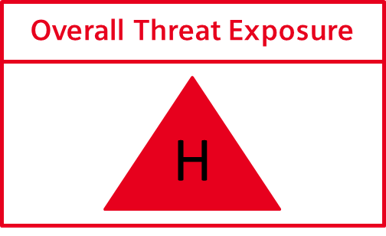
\includegraphics{Images/HighThreat.png}} 
% 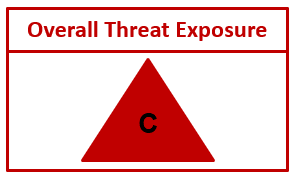
\includegraphics{Images/CriticalThreat.png}, 
% 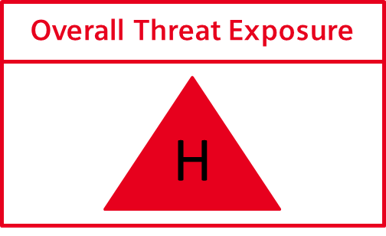
\includegraphics{Images/HighThreat.png}, 
% \includegraphics{Images/MediumThreat.png}, 
% 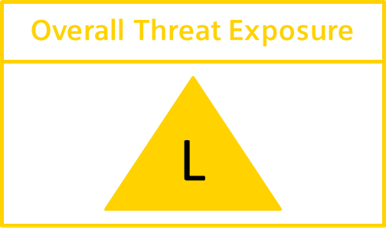
\includegraphics{Images/LowThreat.png}

\newcommand{\FindingsCountCritical}{0}
\newcommand{\FindingsCountHigh}{1}
\newcommand{\FindingsCountMedium}{2}
\newcommand{\FindingsCountLow}{2}
\newcommand{\FindingsCountInfo}{2}
\newcommand{\FindingsCountTotal}{7}
    %
%		File:		Scope_Procedures.tex
%		Author: 	Dusan Repel (SHS TE DC CYS CSA)
%		Date:		02/09/2020
%
%
\clearpage

\SetScopeAndProceduresSection


\end{document}}



%\setlength\cftbeforechapskip{100pt}
%\renewcommand\cftfigafterpnum{\vskip5pt\par}
%\renewcommand\cfttabafterpnum{\vskip5pt\par}


%----------------------------------------------------------------------------------------
%	BUILD REPORT DOCUMENT
%----------------------------------------------------------------------------------------
\newcommand{\ReportDocument}{
    \begin{document}
	\nobibliography*
    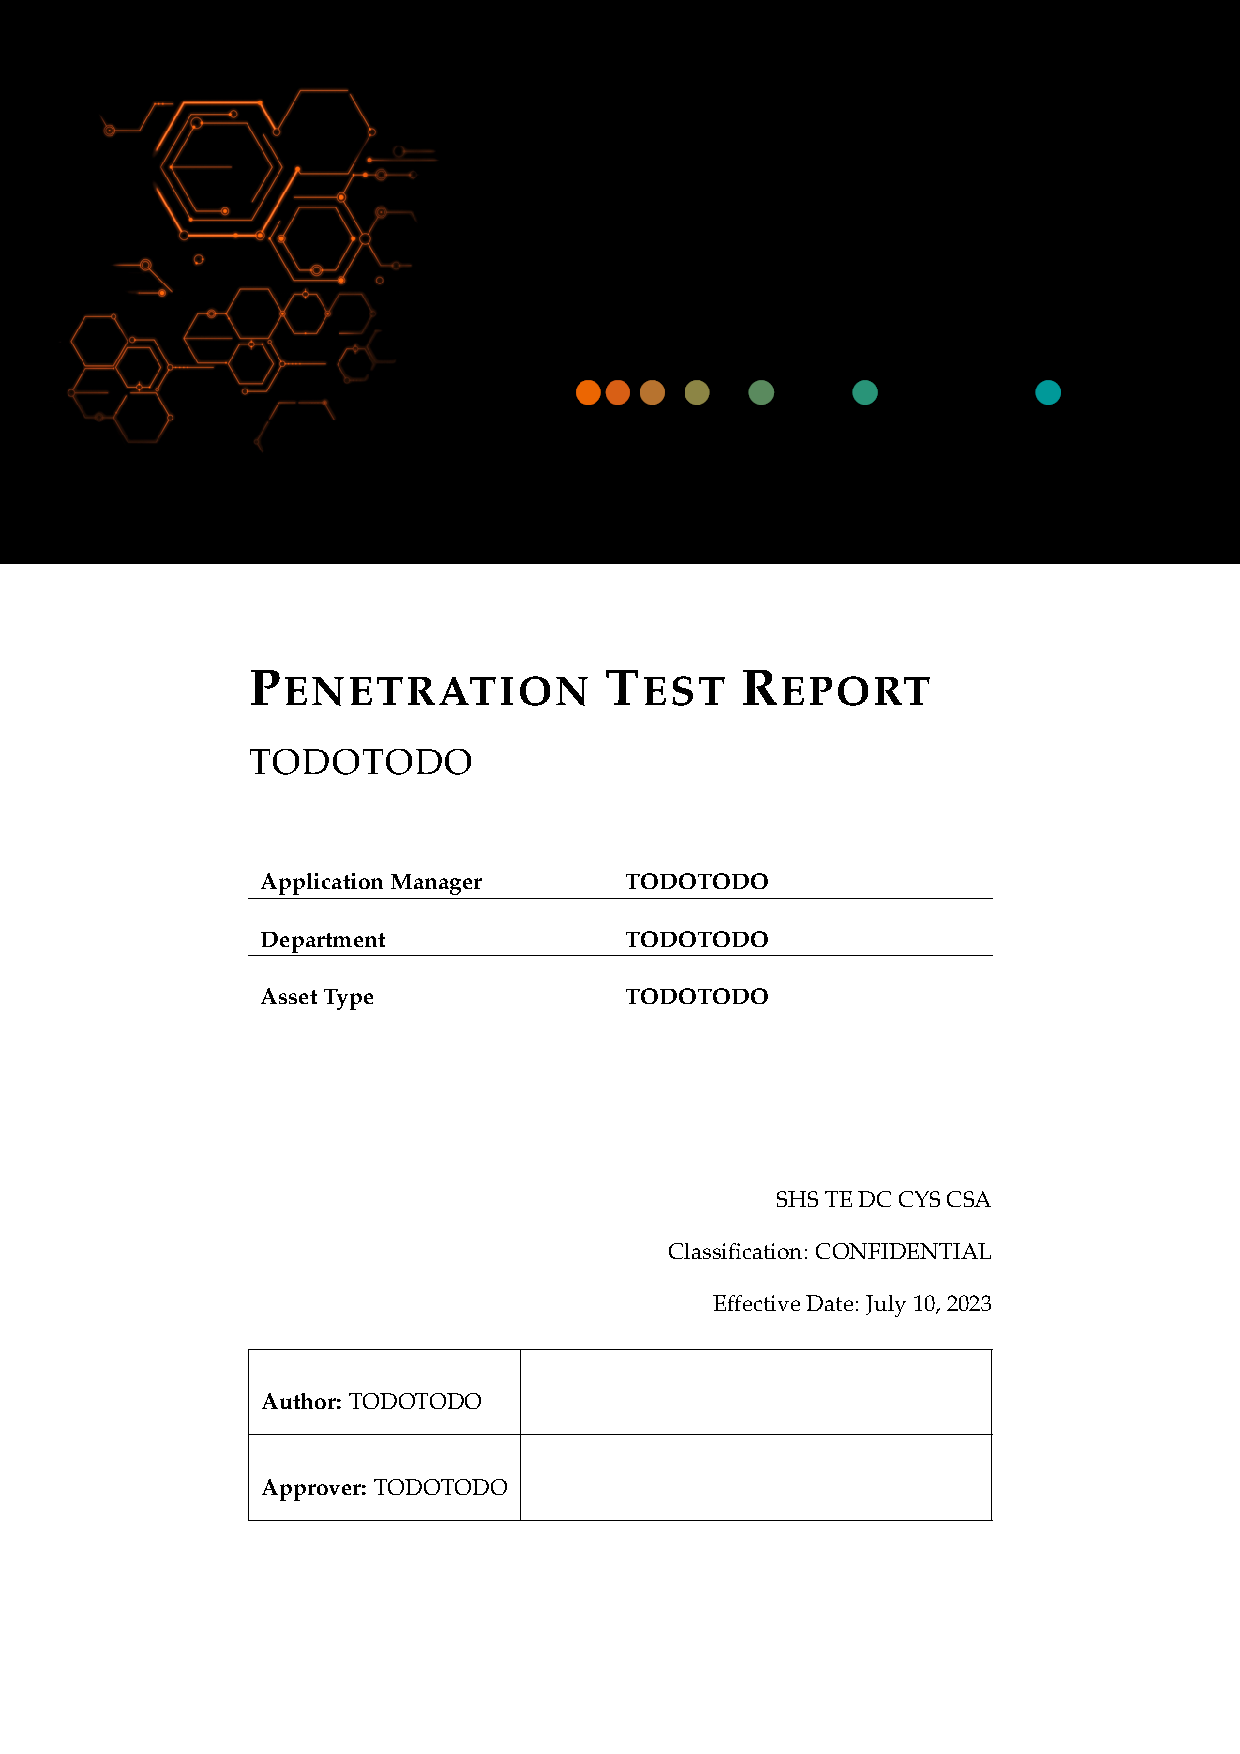
\includepdf{./TitlePage/TitlePage.pdf}
	
	\setlength{\parindent}{0pt}
    \addtolength{\parskip}{8pt}
	
    %----------------------------------------------------------------------------------------
%	DOCUMENT TYPE
%----------------------------------------------------------------------------------------

% Use "\ReportDocument" & "\TitlePageTableReport" when writing Report 
% Use "\ScopeDocument" & "\TitlePageTableScope" for creating Scope Document
\newcommand{\DocumentType}{\ReportDocument}
\renewcommand{\SetTitlePageTable}{\TitlePageTableReport}

%----------------------------------------------------------------------------------------
%	TITLE PAGE
%----------------------------------------------------------------------------------------
\newcommand{\ReportProjectName}{\xspace}
\newcommand{\ReportProjectType}{\xspace}
\newcommand{\AssetType}{\xspace}

%----------------------------------------------------------------------------------------
%	AUTHORS, REVIEWERS, APPROVERS
%----------------------------------------------------------------------------------------
\newcommand{\ReportDocumentMainAuthor}{Lukas Nad}
\newcommand{\ReportDocumentAuthor}{Lukas Nad}
\newcommand{\ReportDocumentReviewer}{}
\newcommand{\ReportDocumentApprover}{Filip Mrocek}

%----------------------------------------------------------------------------------------
%	DOCUMENT VERSION HISTORY
%----------------------------------------------------------------------------------------
% Document version history. Copy the inner line for subsequent version entries.
% Example: \ReportVersionEntry{DATE}{VERSION}{FIRSTNAME LASTNAME}{draft / review / released}{COMMENT}

% TODO: investigate git version tags (automatic compilation of document history table)

\newcommand{\ReportDocumentHistory}{
}


%----------------------------------------------------------------------------------------
%	GENERAL DOCUMENT INFORMATION
%----------------------------------------------------------------------------------------
\newcommand{\FiscalYear}{}
\newcommand{\ReportVersion}{Default}
\newcommand{\ReportDate}{June 12, 2023}
\newcommand{\ReportDocumentClassification}{CONFIDENTIAL}

\newcommand{\ReportStatus}{} 
% \newcommand{\ReportStatus}{DRAFT} 
    {
		% Use ToC depth level=1
		\setcounter{tocdepth}{1}
		
        \hypersetup{linkcolor=blue}
        \tableofcontents
		%\addcontentsline{toc}{chapter}{List of Figures}
        %\listoffigures
        %\addcontentsline{toc}{chapter}{List of Tables}
		%\listoftables
    }   
    
	
    %
%		File:		Disclaimer.tex
%		Author: 	Dusan Repel (SHS TE DC CYS CSA)
%		Date:		02/09/2020
%
%
\clearpage

\chapter{Disclaimer}
\label{chapter:Disclaimer}

\small
\noindent Please note the following aspects of this penetration test:

\begin{itemize}
    %
    \item	 Lorem ipsum dolor sit amet, consectetur adipiscing elit. Donec lacinia tellus sed dui accumsan placerat sed ut lorem. Cras aliquet. 
    
    \item	 Lorem ipsum dolor sit amet, consectetur adipiscing elit. Donec lacinia tellus sed dui accumsan placerat sed ut lorem. Cras aliquet. 
    
    \item	 Lorem ipsum dolor sit amet, consectetur adipiscing elit. Donec lacinia tellus sed dui accumsan placerat sed ut lorem. Cras aliquet. 
    
    \item	 Lorem ipsum dolor sit amet, consectetur adipiscing elit. Donec lacinia tellus sed dui accumsan placerat sed ut lorem. Cras aliquet. 
    
    \item	 	Lorem ipsum dolor sit amet, consectetur adipiscing elit. Donec lacinia tellus sed dui accumsan placerat sed ut lorem. Cras aliquet. 
    
    \item	 	Lorem ipsum dolor sit amet, consectetur adipiscing elit. Donec lacinia tellus sed dui accumsan placerat sed ut lorem. Cras aliquet. 
    
    \item	 	Lorem ipsum dolor sit amet, consectetur adipiscing elit. Donec lacinia tellus sed dui accumsan placerat sed ut lorem. Cras aliquet. 
    
    \item	 	Lorem ipsum dolor sit amet, consectetur adipiscing elit. Donec lacinia tellus sed dui accumsan placerat sed ut lorem. Cras aliquet. 
    
    \item	 	Lorem ipsum dolor sit amet, consectetur adipiscing elit. Donec lacinia tellus sed dui accumsan placerat sed ut lorem. Cras aliquet. 
    
    \item	 	Lorem ipsum dolor sit amet, consectetur adipiscing elit. Donec lacinia tellus sed dui accumsan placerat sed ut lorem. Cras aliquet. 
    
    \end{itemize}
    %----------------------------------------------------------------------------------------
%	EXECUTIVE SUMMARY
%----------------------------------------------------------------------------------------
%-<ExecSum>->

The Penetration Testing team at SHS TE DC CYS CSA in Slovakia conducted a penetration test of \textbf{\textsc{\ReportProjectName}} system in order to assess its overall security posture. Lorem ipsum dolor sit amet, consectetur adipiscing elit. Sed ultricies pharetra pretium. Cras varius purus eu cursus vehicula. Sed in molestie arcu, id placerat velit. Praesent sagittis purus in neque convallis, a faucibus odio egestas. Nam ultrices, metus et mattis facilisis, felis lectus tempor velit, a interdum nisl libero nec dui. Mauris interdum scelerisque semper. Cras mattis id lacus a ullamcorper. Curabitur fermentum vehicula leo, vel convallis turpis luctus nec. In mollis vitae diam in ornare. Donec molestie augue nisl, malesuada maximus urna gravida quis. Curabitur ac ante turpis. Nulla facilisi. Aenean eleifend ipsum at velit lobortis, in hendrerit arcu dapibus. Proin ut lacus sed tellus maximus euismod. Suspendisse elementum mauris tellus, eget imperdiet leo dictum nec. Fusce tortor mauris, iaculis non tristique ut, condimentum a odio.Maecenas tincidunt sollicitudin metus id eleifend. Cras justo urna, tempus et mi vestibulum, iaculis pellentesque nunc. Etiam nisi nibh, bibendum sed augue in, molestie lacinia turpis. Ut bibendum pretium mi vel volutpat. Praesent mattis scelerisque neque a vehicula. Cras nec iaculis mi, in rutrum ligula. Suspendisse potenti.Fusce mollis, erat eget tempus ornare, erat nisl mattis dolor, sed porta mauris quam eget tortor. Etiam bibendum sodales lorem ut fringilla. Phasellus in urna ex. In venenatis turpis a augue egestas efficitur. Interdum et malesuada fames ac ante ipsum primis in faucibus. Cras laoreet odio eu auctor molestie. In congue malesuada sollicitudin.Integer egestas mollis ex quis semper. Nam vitae diam aliquet, elementum leo molestie, suscipit mauris. Suspendisse ex magna, fermentum eu sem non, convallis faucibus nisl. In id dignissim orci, non sodales ante. Nulla bibendum sem nec turpis porta pulvinar. Curabitur fringilla libero ut ex faucibus, non ultrices nisl volutpat. Quisque imperdiet condimentum diam eu scelerisque. Integer ullamcorper euismod accumsan. Curabitur efficitur, neque non blandit tempus, quam erat viverra risus, eu placerat risus elit eu neque. 

%-<ExecSum>
\pagebreak
\section*{Overall Exposure}
    %----------------------------------------------------------------------------------------
%	PROJECT INFORMATION
%----------------------------------------------------------------------------------------
\newcommand{\ApplicationManager}{Anakin Skywalker}
\newcommand{\ApplicationManagerDepartment}{SHS DI D\&A CEC ITH EH-PLM}
\newcommand{\ApplicationManagerContact}{\href{mailto://anakin.skywalker@siemens-healthineers.com}{anakin.skywalker\footnotemark[1]}}

\newcommand{\BusinessOwnerName}{Padme Amidala}
\newcommand{\BusinessOwnerDepartment}{SHS DI D\&A CEC EPE}
\newcommand{\BusinessOwnerContact}{\href{mailto://padme.amidala@siemens-healthineers.com}{padme.amidala\footnotemark[1]}}

\newcommand{\BusinessRepresentativeName}{Luke Skywalker}
\newcommand{\BusinessRepresentativeDepartment}{SHS DI D\&A CEC ITH EH-PLM}
\newcommand{\BusinessRepresentativeContact}{\href{mailto://luke.skywalker@siemens-healthineers.com}{luke.skywalker\footnotemark[1]}}

\newcommand{\TechnicalContactsNumber}{2}
\newcommand{\TechnicalContacts}{
	Obi Wan Kenobi &  SHS TE DC SVK D\&A DIG PTM & \href{mailto://obi-wan.kenobi@siemens-healthineers.com}{obi-wan.kenobi\footnotemark[1]} \\
	& Baby Yoda  & SHS DI D\&A CEC ITH EH-R\&D & \href{mailto://baby.yoda@siemens-healthineers.com}{baby.yoda\footnotemark[1]} \\
}

% Not needed for Scope document
% Required for Report document
\newcommand{\PentestLeadName}{Lukas Nad}
\newcommand{\PentestLeadDepartment}{SHS TE DC CYS CSA P\&PA}
\newcommand{\PentestLeadContact}{\href{mailto://lukas.nad@siemens-healthineers.com}{lukas.nad\footnotemark[1]}}

\newcommand{\PentestCoordinatorName}{Alzbeta Vojtusova}
\newcommand{\PentestCoordinatorDepartment}{SHS TE DC CYS CSA P\&PA}
\newcommand{\PentestCoordinatorContact}{\href{mailto://alzbeta.vojtusova@siemens-healthineers.com}{alzbeta.vojtusova\footnotemark[1]}}



\newcommand{\PentestParticipantsNumber}{3} % Number of participants in "Penetration Testing Team"
\newcommand{\PentestTeamMember}{
	\LukasN			\\ &
	Michal Olencin & SHS TE DC CYS CSA P\&PA & \href{mailto://michal.olencin@siemens-healthineers.com}{michal.olencin\footnotemark[1]}}		\\ &
	\TakshM			\\
	}

%----------------------------------------------------------------------------------------
%	TARGET INFORMATION
%----------------------------------------------------------------------------------------
\newcommand{\TargetInfoName}{\ReportProjectName} %% Asset Name
\newcommand{\TargetInfoVersion}{12.1.1.2} %% Asset Version 	
\newcommand{\TargetInfoType}{\AssetType} %% Asset Type
\newcommand{\TargetInfoEnvironment}{Testing Environment}
\newcommand{\TargetInfoInternetFacing}{Yes} %% Asset Internet Facing
\newcommand{\TargetInfoSNXConnectivity}{No} %% SNX Connectivity
\newcommand{\TargetInfoHostingLocation}{Special Network} %% Hosting Location
\newcommand{\TargetInfoHostingProvider}{N/A} %% Hosting Provider
\newcommand{\TargetInfoLifecyclePhase}{Pre-Production}
\newcommand{\TargetInfoCriticality}{N/A}
\newcommand{\TargetInfoAssetID}{N/A}
\newcommand{\TargetInfoSHARPUUID}{N/A} %% SHARP UUID
\newcommand{\TargetInfoDescription}{Lorem ipsum dolor sit amet, consectetur adipiscing elit. Sed ultricies pharetra pretium. Cras varius purus eu cursus vehicula. Sed in molestie arcu, id placerat velit. Praesent sagittis purus in neque convallis, a faucibus odio egestas. Nam ultrices, metus et mattis facilisis, felis lectus tempor velit, a interdum nisl libero nec dui. Mauris interdum scelerisque semper. Cras mattis id lacus a ullamcorper. Curabitur fermentum vehicula leo, vel convallis turpis luctus nec. In mollis vitae diam in ornare. Donec molestie augue nisl, malesuada maximus urna gravida quis. Curabitur ac ante turpis. Nulla facilisi. Aenean eleifend ipsum at velit lobortis, in hendrerit arcu dapibus. Proin ut lacus sed tellus maximus euismod. Suspendisse elementum mauris tellus, eget imperdiet leo dictum nec. Fusce tortor mauris, iaculis non tristique ut, condimentum a odio.}

%----------------------------------------------------------------------------------------
%	AGREED TIMEFRAME
%----------------------------------------------------------------------------------------
\newcommand{\TimeframeTotal}{10 working days} 
\newcommand{\TimeframeStart}{2023-05-29} 
\newcommand{\TimeframeEnd}{2023-06-09} 
\newcommand{\TimeframeReportDue}{2023-06-12} 
\newcommand{\TimeframeComment}{-}

%----------------------------------------------------------------------------------------
%	FINDINGS COUNT AND OVERALL THREAT EXPOSURE
%----------------------------------------------------------------------------------------
% Not needed for Scope document
% Required for Report document

\newcommand{\OverallThreatExposureImage}{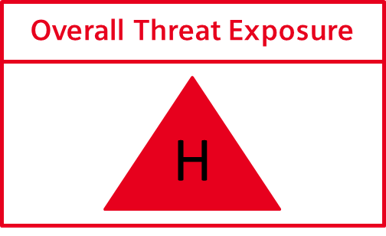
\includegraphics{Images/HighThreat.png}} 
% 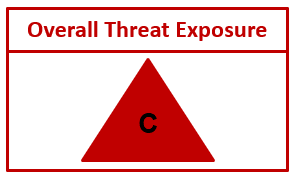
\includegraphics{Images/CriticalThreat.png}, 
% 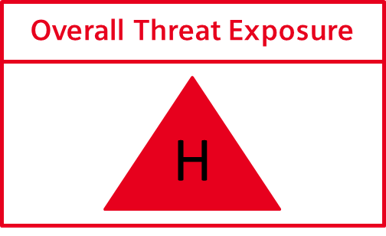
\includegraphics{Images/HighThreat.png}, 
% \includegraphics{Images/MediumThreat.png}, 
% 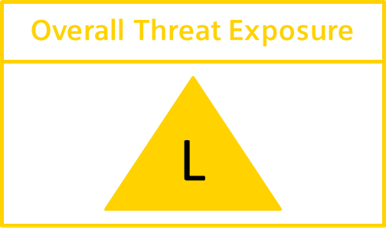
\includegraphics{Images/LowThreat.png}

\newcommand{\FindingsCountCritical}{0}
\newcommand{\FindingsCountHigh}{1}
\newcommand{\FindingsCountMedium}{2}
\newcommand{\FindingsCountLow}{2}
\newcommand{\FindingsCountInfo}{2}
\newcommand{\FindingsCountTotal}{7}
    \chapter{Summary of Findings}
\renewcommand{\ReportBoolWriteSummary}{true}
\IfFileExists{\ReportSummaryFile}{\input{\ReportSummaryFile}}{}
\renewcommand{\ReportBoolWriteSummary}{false}
    
\clearpage
\chapter{Findings}

\renewcommand{\FindingNumber}{1}
\renewcommand{\ReportBoolIsFirstFindingInSection}{true}
\immediate\openout\outfileSummary=\ReportSummaryFile
%
%		File:		./Config/Findings_Database
%		Author: 	Dusan Repel (SHS TE DC CYS CSA)
%		Date:		02/06/2021
%
%		Draft: everyone can group their findings together.
%		Release: the lines will be re-ordered after ranking according to criticality.
%


% CRIT

% HIGH

%
%
%		Finding: Template
%		Author: the DR
%
%
\renewcommand{\FindingAuthor}{Taksh Medhavi}
% DO NOT USE \par, \newline or any other line breaking command in FindingName => report will not build
\renewcommand{\FindingName}{ePHI is stored on device without encryption}
\renewcommand{\Location}{dummyapplication.apk}
\renewcommand{\Component}{Android local storage}
\renewcommand{\FoundWith}{TODOTODO}
\renewcommand{\TestMethod}{TODOTODO}
\renewcommand{\CVSS}{8.0}
\renewcommand{\CVSSvector}{CVSS:3.1/AV:A/AC:L/PR:L/UI:N/S:U/C:H/I:H/A:H}
\renewcommand{\CWE}{359}
% Poor-man's combo boxes:
% High, Medium, Low, Info, TBR (To Be Rated)
\renewcommand{\Criticality}{High}
% Easy, Average, Hard, TBR (To Be Rated)
\renewcommand{\Exploitability}{Easy}
% Access control, Application Design, Information Disclosure, Outdated Software, Security Configuration
\renewcommand{\Category}{Application Design}
% Easy, Average, Difficult, TBR (To Be Rated)
\renewcommand{\Detectability}{Easy}


\ReportFindingHeader{\FindingName}


%-------------------------------------------
%	Details                                |
%-------------------------------------------

\subsection*{Details}

Application allows user to save ePHI (Electronic Protected Health Information) on device and patient information is stored in plain text in HTML file format. Application stores HTML file in \texttt{android > data > com.siemenshealthineers.dummyapplicationapp > files} directory. The file contains sensitive information such as patient vitals, allergies, diagnostic results and medication in it.


%-<Details>
%-------------------------------------------
%	Impact                                 |
%-------------------------------------------

\subsection*{Impact}

Third party application installed in mobile devices can access ePHI stored in application data directory and since data at rest is stored without encryption, attacker can read contents of file which can lead to loss of confidentiality and violation of healthcare compliance. Application with external storage read/write permission can affect file integrity, as well as, application availability. In another scenario, attacker with local access of device can use file manager to access patient data. 

%-<Impact>
%-------------------------------------------
%	Repeatability                          |
%-------------------------------------------

\newpage
\subsection*{Repeatability}

User can download patient summary details in device in plaintext HTML file as shown in \cref{figure:003.ephi_2.jpg}. \cref{figure:005.ephi_in_html_file} shows that HTML file contains ePHI such as patient vitals, allergies, diagnostic results and medication in it.

\begin{figure}[h]
	\begin{subfigure}{0.5\textwidth}
	
\includegraphics[width=0.9\linewidth]{\CurrentFilePath/ProperScreenshot.png} 
	\caption{Downloading patient information}
	\label{figure:003.ephi_2.jpg}
	\end{subfigure}
	\begin{subfigure}{0.5\textwidth}
	
\includegraphics[width=0.9\linewidth]{\CurrentFilePath/ProperScreenshot.png}
	\caption{ePHI in plaintext HTML file}
	\label{figure:005.ephi_in_html_file}
	\end{subfigure}
	\caption{ePHI without data at rest encryption}
	\label{fig:005.ephi_in_html_file}
\end{figure}

\newpage

User can also open patient summary HTML file using file manager and access ePHI as shown in \cref{figure:006.patient_data_file_location}.

\begin{figure}[H]
\centering

\includegraphics[scale=1.0,frame]{\CurrentFilePath/ProperScreenshot.png}
\caption{EPHI access via file manager}
\label{figure:006.patient_data_file_location}
\end{figure}




 
%-<Repeatability>
%-------------------------------------------
%	Countermeasures                        |
%-------------------------------------------

\subsection*{Countermeasures}

Application allows ePHI to be downloaded in plain HTML without encryption at rest. Application should handle patient data as per healthcare compliances applicable and should provide PDF report with password.


%-<Countermeasures>
%-------------------------------------------
%	References - pulls bib entries         |
%-------------------------------------------

\subsection*{References}

This finding references the following information sources:

\begin{itemize}
	\item \href{https://www.first.org/cvss/calculator/3.0#CVSS:3.0/AV:A/AC:L/PR:L/UI:N/S:U/C:H/I:H/A:H}
	{CVSS 8.0}
	% \item \href{https://cwe.mitre.org/data/definitions/359.html}
	% {CWE-359}
	\item \bibentry{CWE-359}
\end{itemize}

%-<References>



% MED
%
%
%		Finding: Template
%		Author: the DR
%
%
\renewcommand{\FindingAuthor}{Taksh Medhavi}
% DO NOT USE \par, \newline or any other line breaking command in FindingName => report will not build
\renewcommand{\FindingName}{ePHI is stored on device without encryption}
\renewcommand{\Location}{dummyapplication.apk}
\renewcommand{\Component}{Android local storage}
\renewcommand{\FoundWith}{TODOTODO}
\renewcommand{\TestMethod}{TODOTODO}
\renewcommand{\CVSS}{8.0}
\renewcommand{\CVSSvector}{CVSS:3.1/AV:A/AC:L/PR:L/UI:N/S:U/C:H/I:H/A:H}
\renewcommand{\CWE}{359}
% Poor-man's combo boxes:
% High, Medium, Low, Info, TBR (To Be Rated)
\renewcommand{\Criticality}{High}
% Easy, Average, Hard, TBR (To Be Rated)
\renewcommand{\Exploitability}{Easy}
% Access control, Application Design, Information Disclosure, Outdated Software, Security Configuration
\renewcommand{\Category}{Application Design}
% Easy, Average, Difficult, TBR (To Be Rated)
\renewcommand{\Detectability}{Easy}


\ReportFindingHeader{\FindingName}


%-------------------------------------------
%	Details                                |
%-------------------------------------------

\subsection*{Details}

Application allows user to save ePHI (Electronic Protected Health Information) on device and patient information is stored in plain text in HTML file format. Application stores HTML file in \texttt{android > data > com.siemenshealthineers.dummyapplicationapp > files} directory. The file contains sensitive information such as patient vitals, allergies, diagnostic results and medication in it.


%-<Details>
%-------------------------------------------
%	Impact                                 |
%-------------------------------------------

\subsection*{Impact}

Third party application installed in mobile devices can access ePHI stored in application data directory and since data at rest is stored without encryption, attacker can read contents of file which can lead to loss of confidentiality and violation of healthcare compliance. Application with external storage read/write permission can affect file integrity, as well as, application availability. In another scenario, attacker with local access of device can use file manager to access patient data. 

%-<Impact>
%-------------------------------------------
%	Repeatability                          |
%-------------------------------------------

\newpage
\subsection*{Repeatability}

User can download patient summary details in device in plaintext HTML file as shown in \cref{figure:003.ephi_2.jpg}. \cref{figure:005.ephi_in_html_file} shows that HTML file contains ePHI such as patient vitals, allergies, diagnostic results and medication in it.

\begin{figure}[h]
	\begin{subfigure}{0.5\textwidth}
	
\includegraphics[width=0.9\linewidth]{\CurrentFilePath/ProperScreenshot.png} 
	\caption{Downloading patient information}
	\label{figure:003.ephi_2.jpg}
	\end{subfigure}
	\begin{subfigure}{0.5\textwidth}
	
\includegraphics[width=0.9\linewidth]{\CurrentFilePath/ProperScreenshot.png}
	\caption{ePHI in plaintext HTML file}
	\label{figure:005.ephi_in_html_file}
	\end{subfigure}
	\caption{ePHI without data at rest encryption}
	\label{fig:005.ephi_in_html_file}
\end{figure}

\newpage

User can also open patient summary HTML file using file manager and access ePHI as shown in \cref{figure:006.patient_data_file_location}.

\begin{figure}[H]
\centering

\includegraphics[scale=1.0,frame]{\CurrentFilePath/ProperScreenshot.png}
\caption{EPHI access via file manager}
\label{figure:006.patient_data_file_location}
\end{figure}




 
%-<Repeatability>
%-------------------------------------------
%	Countermeasures                        |
%-------------------------------------------

\subsection*{Countermeasures}

Application allows ePHI to be downloaded in plain HTML without encryption at rest. Application should handle patient data as per healthcare compliances applicable and should provide PDF report with password.


%-<Countermeasures>
%-------------------------------------------
%	References - pulls bib entries         |
%-------------------------------------------

\subsection*{References}

This finding references the following information sources:

\begin{itemize}
	\item \href{https://www.first.org/cvss/calculator/3.0#CVSS:3.0/AV:A/AC:L/PR:L/UI:N/S:U/C:H/I:H/A:H}
	{CVSS 8.0}
	% \item \href{https://cwe.mitre.org/data/definitions/359.html}
	% {CWE-359}
	\item \bibentry{CWE-359}
\end{itemize}

%-<References>

 % 4.0

%
%
%		Finding: Template
%		Author: the DR
%
%
\renewcommand{\FindingAuthor}{Taksh Medhavi}
% DO NOT USE \par, \newline or any other line breaking command in FindingName => report will not build
\renewcommand{\FindingName}{ePHI is stored on device without encryption}
\renewcommand{\Location}{dummyapplication.apk}
\renewcommand{\Component}{Android local storage}
\renewcommand{\FoundWith}{TODOTODO}
\renewcommand{\TestMethod}{TODOTODO}
\renewcommand{\CVSS}{8.0}
\renewcommand{\CVSSvector}{CVSS:3.1/AV:A/AC:L/PR:L/UI:N/S:U/C:H/I:H/A:H}
\renewcommand{\CWE}{359}
% Poor-man's combo boxes:
% High, Medium, Low, Info, TBR (To Be Rated)
\renewcommand{\Criticality}{High}
% Easy, Average, Hard, TBR (To Be Rated)
\renewcommand{\Exploitability}{Easy}
% Access control, Application Design, Information Disclosure, Outdated Software, Security Configuration
\renewcommand{\Category}{Application Design}
% Easy, Average, Difficult, TBR (To Be Rated)
\renewcommand{\Detectability}{Easy}


\ReportFindingHeader{\FindingName}


%-------------------------------------------
%	Details                                |
%-------------------------------------------

\subsection*{Details}

Application allows user to save ePHI (Electronic Protected Health Information) on device and patient information is stored in plain text in HTML file format. Application stores HTML file in \texttt{android > data > com.siemenshealthineers.dummyapplicationapp > files} directory. The file contains sensitive information such as patient vitals, allergies, diagnostic results and medication in it.


%-<Details>
%-------------------------------------------
%	Impact                                 |
%-------------------------------------------

\subsection*{Impact}

Third party application installed in mobile devices can access ePHI stored in application data directory and since data at rest is stored without encryption, attacker can read contents of file which can lead to loss of confidentiality and violation of healthcare compliance. Application with external storage read/write permission can affect file integrity, as well as, application availability. In another scenario, attacker with local access of device can use file manager to access patient data. 

%-<Impact>
%-------------------------------------------
%	Repeatability                          |
%-------------------------------------------

\newpage
\subsection*{Repeatability}

User can download patient summary details in device in plaintext HTML file as shown in \cref{figure:003.ephi_2.jpg}. \cref{figure:005.ephi_in_html_file} shows that HTML file contains ePHI such as patient vitals, allergies, diagnostic results and medication in it.

\begin{figure}[h]
	\begin{subfigure}{0.5\textwidth}
	
\includegraphics[width=0.9\linewidth]{\CurrentFilePath/ProperScreenshot.png} 
	\caption{Downloading patient information}
	\label{figure:003.ephi_2.jpg}
	\end{subfigure}
	\begin{subfigure}{0.5\textwidth}
	
\includegraphics[width=0.9\linewidth]{\CurrentFilePath/ProperScreenshot.png}
	\caption{ePHI in plaintext HTML file}
	\label{figure:005.ephi_in_html_file}
	\end{subfigure}
	\caption{ePHI without data at rest encryption}
	\label{fig:005.ephi_in_html_file}
\end{figure}

\newpage

User can also open patient summary HTML file using file manager and access ePHI as shown in \cref{figure:006.patient_data_file_location}.

\begin{figure}[H]
\centering

\includegraphics[scale=1.0,frame]{\CurrentFilePath/ProperScreenshot.png}
\caption{EPHI access via file manager}
\label{figure:006.patient_data_file_location}
\end{figure}




 
%-<Repeatability>
%-------------------------------------------
%	Countermeasures                        |
%-------------------------------------------

\subsection*{Countermeasures}

Application allows ePHI to be downloaded in plain HTML without encryption at rest. Application should handle patient data as per healthcare compliances applicable and should provide PDF report with password.


%-<Countermeasures>
%-------------------------------------------
%	References - pulls bib entries         |
%-------------------------------------------

\subsection*{References}

This finding references the following information sources:

\begin{itemize}
	\item \href{https://www.first.org/cvss/calculator/3.0#CVSS:3.0/AV:A/AC:L/PR:L/UI:N/S:U/C:H/I:H/A:H}
	{CVSS 8.0}
	% \item \href{https://cwe.mitre.org/data/definitions/359.html}
	% {CWE-359}
	\item \bibentry{CWE-359}
\end{itemize}

%-<References>



% LOW
%
%
%		Finding: Template
%		Author: the DR
%
%
\renewcommand{\FindingAuthor}{Taksh Medhavi}
% DO NOT USE \par, \newline or any other line breaking command in FindingName => report will not build
\renewcommand{\FindingName}{ePHI is stored on device without encryption}
\renewcommand{\Location}{dummyapplication.apk}
\renewcommand{\Component}{Android local storage}
\renewcommand{\FoundWith}{TODOTODO}
\renewcommand{\TestMethod}{TODOTODO}
\renewcommand{\CVSS}{8.0}
\renewcommand{\CVSSvector}{CVSS:3.1/AV:A/AC:L/PR:L/UI:N/S:U/C:H/I:H/A:H}
\renewcommand{\CWE}{359}
% Poor-man's combo boxes:
% High, Medium, Low, Info, TBR (To Be Rated)
\renewcommand{\Criticality}{High}
% Easy, Average, Hard, TBR (To Be Rated)
\renewcommand{\Exploitability}{Easy}
% Access control, Application Design, Information Disclosure, Outdated Software, Security Configuration
\renewcommand{\Category}{Application Design}
% Easy, Average, Difficult, TBR (To Be Rated)
\renewcommand{\Detectability}{Easy}


\ReportFindingHeader{\FindingName}


%-------------------------------------------
%	Details                                |
%-------------------------------------------

\subsection*{Details}

Application allows user to save ePHI (Electronic Protected Health Information) on device and patient information is stored in plain text in HTML file format. Application stores HTML file in \texttt{android > data > com.siemenshealthineers.dummyapplicationapp > files} directory. The file contains sensitive information such as patient vitals, allergies, diagnostic results and medication in it.


%-<Details>
%-------------------------------------------
%	Impact                                 |
%-------------------------------------------

\subsection*{Impact}

Third party application installed in mobile devices can access ePHI stored in application data directory and since data at rest is stored without encryption, attacker can read contents of file which can lead to loss of confidentiality and violation of healthcare compliance. Application with external storage read/write permission can affect file integrity, as well as, application availability. In another scenario, attacker with local access of device can use file manager to access patient data. 

%-<Impact>
%-------------------------------------------
%	Repeatability                          |
%-------------------------------------------

\newpage
\subsection*{Repeatability}

User can download patient summary details in device in plaintext HTML file as shown in \cref{figure:003.ephi_2.jpg}. \cref{figure:005.ephi_in_html_file} shows that HTML file contains ePHI such as patient vitals, allergies, diagnostic results and medication in it.

\begin{figure}[h]
	\begin{subfigure}{0.5\textwidth}
	
\includegraphics[width=0.9\linewidth]{\CurrentFilePath/ProperScreenshot.png} 
	\caption{Downloading patient information}
	\label{figure:003.ephi_2.jpg}
	\end{subfigure}
	\begin{subfigure}{0.5\textwidth}
	
\includegraphics[width=0.9\linewidth]{\CurrentFilePath/ProperScreenshot.png}
	\caption{ePHI in plaintext HTML file}
	\label{figure:005.ephi_in_html_file}
	\end{subfigure}
	\caption{ePHI without data at rest encryption}
	\label{fig:005.ephi_in_html_file}
\end{figure}

\newpage

User can also open patient summary HTML file using file manager and access ePHI as shown in \cref{figure:006.patient_data_file_location}.

\begin{figure}[H]
\centering

\includegraphics[scale=1.0,frame]{\CurrentFilePath/ProperScreenshot.png}
\caption{EPHI access via file manager}
\label{figure:006.patient_data_file_location}
\end{figure}




 
%-<Repeatability>
%-------------------------------------------
%	Countermeasures                        |
%-------------------------------------------

\subsection*{Countermeasures}

Application allows ePHI to be downloaded in plain HTML without encryption at rest. Application should handle patient data as per healthcare compliances applicable and should provide PDF report with password.


%-<Countermeasures>
%-------------------------------------------
%	References - pulls bib entries         |
%-------------------------------------------

\subsection*{References}

This finding references the following information sources:

\begin{itemize}
	\item \href{https://www.first.org/cvss/calculator/3.0#CVSS:3.0/AV:A/AC:L/PR:L/UI:N/S:U/C:H/I:H/A:H}
	{CVSS 8.0}
	% \item \href{https://cwe.mitre.org/data/definitions/359.html}
	% {CWE-359}
	\item \bibentry{CWE-359}
\end{itemize}

%-<References>

 % 3.3
%
%
%		Finding: Template
%		Author: the DR
%
%
\renewcommand{\FindingAuthor}{Taksh Medhavi}
% DO NOT USE \par, \newline or any other line breaking command in FindingName => report will not build
\renewcommand{\FindingName}{ePHI is stored on device without encryption}
\renewcommand{\Location}{dummyapplication.apk}
\renewcommand{\Component}{Android local storage}
\renewcommand{\FoundWith}{TODOTODO}
\renewcommand{\TestMethod}{TODOTODO}
\renewcommand{\CVSS}{8.0}
\renewcommand{\CVSSvector}{CVSS:3.1/AV:A/AC:L/PR:L/UI:N/S:U/C:H/I:H/A:H}
\renewcommand{\CWE}{359}
% Poor-man's combo boxes:
% High, Medium, Low, Info, TBR (To Be Rated)
\renewcommand{\Criticality}{High}
% Easy, Average, Hard, TBR (To Be Rated)
\renewcommand{\Exploitability}{Easy}
% Access control, Application Design, Information Disclosure, Outdated Software, Security Configuration
\renewcommand{\Category}{Application Design}
% Easy, Average, Difficult, TBR (To Be Rated)
\renewcommand{\Detectability}{Easy}


\ReportFindingHeader{\FindingName}


%-------------------------------------------
%	Details                                |
%-------------------------------------------

\subsection*{Details}

Application allows user to save ePHI (Electronic Protected Health Information) on device and patient information is stored in plain text in HTML file format. Application stores HTML file in \texttt{android > data > com.siemenshealthineers.dummyapplicationapp > files} directory. The file contains sensitive information such as patient vitals, allergies, diagnostic results and medication in it.


%-<Details>
%-------------------------------------------
%	Impact                                 |
%-------------------------------------------

\subsection*{Impact}

Third party application installed in mobile devices can access ePHI stored in application data directory and since data at rest is stored without encryption, attacker can read contents of file which can lead to loss of confidentiality and violation of healthcare compliance. Application with external storage read/write permission can affect file integrity, as well as, application availability. In another scenario, attacker with local access of device can use file manager to access patient data. 

%-<Impact>
%-------------------------------------------
%	Repeatability                          |
%-------------------------------------------

\newpage
\subsection*{Repeatability}

User can download patient summary details in device in plaintext HTML file as shown in \cref{figure:003.ephi_2.jpg}. \cref{figure:005.ephi_in_html_file} shows that HTML file contains ePHI such as patient vitals, allergies, diagnostic results and medication in it.

\begin{figure}[h]
	\begin{subfigure}{0.5\textwidth}
	
\includegraphics[width=0.9\linewidth]{\CurrentFilePath/ProperScreenshot.png} 
	\caption{Downloading patient information}
	\label{figure:003.ephi_2.jpg}
	\end{subfigure}
	\begin{subfigure}{0.5\textwidth}
	
\includegraphics[width=0.9\linewidth]{\CurrentFilePath/ProperScreenshot.png}
	\caption{ePHI in plaintext HTML file}
	\label{figure:005.ephi_in_html_file}
	\end{subfigure}
	\caption{ePHI without data at rest encryption}
	\label{fig:005.ephi_in_html_file}
\end{figure}

\newpage

User can also open patient summary HTML file using file manager and access ePHI as shown in \cref{figure:006.patient_data_file_location}.

\begin{figure}[H]
\centering

\includegraphics[scale=1.0,frame]{\CurrentFilePath/ProperScreenshot.png}
\caption{EPHI access via file manager}
\label{figure:006.patient_data_file_location}
\end{figure}




 
%-<Repeatability>
%-------------------------------------------
%	Countermeasures                        |
%-------------------------------------------

\subsection*{Countermeasures}

Application allows ePHI to be downloaded in plain HTML without encryption at rest. Application should handle patient data as per healthcare compliances applicable and should provide PDF report with password.


%-<Countermeasures>
%-------------------------------------------
%	References - pulls bib entries         |
%-------------------------------------------

\subsection*{References}

This finding references the following information sources:

\begin{itemize}
	\item \href{https://www.first.org/cvss/calculator/3.0#CVSS:3.0/AV:A/AC:L/PR:L/UI:N/S:U/C:H/I:H/A:H}
	{CVSS 8.0}
	% \item \href{https://cwe.mitre.org/data/definitions/359.html}
	% {CWE-359}
	\item \bibentry{CWE-359}
\end{itemize}

%-<References>

 % 2.5

% INFO
%
%
%		Finding: Template
%		Author: the DR
%
%
\renewcommand{\FindingAuthor}{Taksh Medhavi}
% DO NOT USE \par, \newline or any other line breaking command in FindingName => report will not build
\renewcommand{\FindingName}{ePHI is stored on device without encryption}
\renewcommand{\Location}{dummyapplication.apk}
\renewcommand{\Component}{Android local storage}
\renewcommand{\FoundWith}{TODOTODO}
\renewcommand{\TestMethod}{TODOTODO}
\renewcommand{\CVSS}{8.0}
\renewcommand{\CVSSvector}{CVSS:3.1/AV:A/AC:L/PR:L/UI:N/S:U/C:H/I:H/A:H}
\renewcommand{\CWE}{359}
% Poor-man's combo boxes:
% High, Medium, Low, Info, TBR (To Be Rated)
\renewcommand{\Criticality}{High}
% Easy, Average, Hard, TBR (To Be Rated)
\renewcommand{\Exploitability}{Easy}
% Access control, Application Design, Information Disclosure, Outdated Software, Security Configuration
\renewcommand{\Category}{Application Design}
% Easy, Average, Difficult, TBR (To Be Rated)
\renewcommand{\Detectability}{Easy}


\ReportFindingHeader{\FindingName}


%-------------------------------------------
%	Details                                |
%-------------------------------------------

\subsection*{Details}

Application allows user to save ePHI (Electronic Protected Health Information) on device and patient information is stored in plain text in HTML file format. Application stores HTML file in \texttt{android > data > com.siemenshealthineers.dummyapplicationapp > files} directory. The file contains sensitive information such as patient vitals, allergies, diagnostic results and medication in it.


%-<Details>
%-------------------------------------------
%	Impact                                 |
%-------------------------------------------

\subsection*{Impact}

Third party application installed in mobile devices can access ePHI stored in application data directory and since data at rest is stored without encryption, attacker can read contents of file which can lead to loss of confidentiality and violation of healthcare compliance. Application with external storage read/write permission can affect file integrity, as well as, application availability. In another scenario, attacker with local access of device can use file manager to access patient data. 

%-<Impact>
%-------------------------------------------
%	Repeatability                          |
%-------------------------------------------

\newpage
\subsection*{Repeatability}

User can download patient summary details in device in plaintext HTML file as shown in \cref{figure:003.ephi_2.jpg}. \cref{figure:005.ephi_in_html_file} shows that HTML file contains ePHI such as patient vitals, allergies, diagnostic results and medication in it.

\begin{figure}[h]
	\begin{subfigure}{0.5\textwidth}
	
\includegraphics[width=0.9\linewidth]{\CurrentFilePath/ProperScreenshot.png} 
	\caption{Downloading patient information}
	\label{figure:003.ephi_2.jpg}
	\end{subfigure}
	\begin{subfigure}{0.5\textwidth}
	
\includegraphics[width=0.9\linewidth]{\CurrentFilePath/ProperScreenshot.png}
	\caption{ePHI in plaintext HTML file}
	\label{figure:005.ephi_in_html_file}
	\end{subfigure}
	\caption{ePHI without data at rest encryption}
	\label{fig:005.ephi_in_html_file}
\end{figure}

\newpage

User can also open patient summary HTML file using file manager and access ePHI as shown in \cref{figure:006.patient_data_file_location}.

\begin{figure}[H]
\centering

\includegraphics[scale=1.0,frame]{\CurrentFilePath/ProperScreenshot.png}
\caption{EPHI access via file manager}
\label{figure:006.patient_data_file_location}
\end{figure}




 
%-<Repeatability>
%-------------------------------------------
%	Countermeasures                        |
%-------------------------------------------

\subsection*{Countermeasures}

Application allows ePHI to be downloaded in plain HTML without encryption at rest. Application should handle patient data as per healthcare compliances applicable and should provide PDF report with password.


%-<Countermeasures>
%-------------------------------------------
%	References - pulls bib entries         |
%-------------------------------------------

\subsection*{References}

This finding references the following information sources:

\begin{itemize}
	\item \href{https://www.first.org/cvss/calculator/3.0#CVSS:3.0/AV:A/AC:L/PR:L/UI:N/S:U/C:H/I:H/A:H}
	{CVSS 8.0}
	% \item \href{https://cwe.mitre.org/data/definitions/359.html}
	% {CWE-359}
	\item \bibentry{CWE-359}
\end{itemize}

%-<References>


%
%
%		Finding: Template
%		Author: the DR
%
%
\renewcommand{\FindingAuthor}{Taksh Medhavi}
% DO NOT USE \par, \newline or any other line breaking command in FindingName => report will not build
\renewcommand{\FindingName}{ePHI is stored on device without encryption}
\renewcommand{\Location}{dummyapplication.apk}
\renewcommand{\Component}{Android local storage}
\renewcommand{\FoundWith}{TODOTODO}
\renewcommand{\TestMethod}{TODOTODO}
\renewcommand{\CVSS}{8.0}
\renewcommand{\CVSSvector}{CVSS:3.1/AV:A/AC:L/PR:L/UI:N/S:U/C:H/I:H/A:H}
\renewcommand{\CWE}{359}
% Poor-man's combo boxes:
% High, Medium, Low, Info, TBR (To Be Rated)
\renewcommand{\Criticality}{High}
% Easy, Average, Hard, TBR (To Be Rated)
\renewcommand{\Exploitability}{Easy}
% Access control, Application Design, Information Disclosure, Outdated Software, Security Configuration
\renewcommand{\Category}{Application Design}
% Easy, Average, Difficult, TBR (To Be Rated)
\renewcommand{\Detectability}{Easy}


\ReportFindingHeader{\FindingName}


%-------------------------------------------
%	Details                                |
%-------------------------------------------

\subsection*{Details}

Application allows user to save ePHI (Electronic Protected Health Information) on device and patient information is stored in plain text in HTML file format. Application stores HTML file in \texttt{android > data > com.siemenshealthineers.dummyapplicationapp > files} directory. The file contains sensitive information such as patient vitals, allergies, diagnostic results and medication in it.


%-<Details>
%-------------------------------------------
%	Impact                                 |
%-------------------------------------------

\subsection*{Impact}

Third party application installed in mobile devices can access ePHI stored in application data directory and since data at rest is stored without encryption, attacker can read contents of file which can lead to loss of confidentiality and violation of healthcare compliance. Application with external storage read/write permission can affect file integrity, as well as, application availability. In another scenario, attacker with local access of device can use file manager to access patient data. 

%-<Impact>
%-------------------------------------------
%	Repeatability                          |
%-------------------------------------------

\newpage
\subsection*{Repeatability}

User can download patient summary details in device in plaintext HTML file as shown in \cref{figure:003.ephi_2.jpg}. \cref{figure:005.ephi_in_html_file} shows that HTML file contains ePHI such as patient vitals, allergies, diagnostic results and medication in it.

\begin{figure}[h]
	\begin{subfigure}{0.5\textwidth}
	
\includegraphics[width=0.9\linewidth]{\CurrentFilePath/ProperScreenshot.png} 
	\caption{Downloading patient information}
	\label{figure:003.ephi_2.jpg}
	\end{subfigure}
	\begin{subfigure}{0.5\textwidth}
	
\includegraphics[width=0.9\linewidth]{\CurrentFilePath/ProperScreenshot.png}
	\caption{ePHI in plaintext HTML file}
	\label{figure:005.ephi_in_html_file}
	\end{subfigure}
	\caption{ePHI without data at rest encryption}
	\label{fig:005.ephi_in_html_file}
\end{figure}

\newpage

User can also open patient summary HTML file using file manager and access ePHI as shown in \cref{figure:006.patient_data_file_location}.

\begin{figure}[H]
\centering

\includegraphics[scale=1.0,frame]{\CurrentFilePath/ProperScreenshot.png}
\caption{EPHI access via file manager}
\label{figure:006.patient_data_file_location}
\end{figure}




 
%-<Repeatability>
%-------------------------------------------
%	Countermeasures                        |
%-------------------------------------------

\subsection*{Countermeasures}

Application allows ePHI to be downloaded in plain HTML without encryption at rest. Application should handle patient data as per healthcare compliances applicable and should provide PDF report with password.


%-<Countermeasures>
%-------------------------------------------
%	References - pulls bib entries         |
%-------------------------------------------

\subsection*{References}

This finding references the following information sources:

\begin{itemize}
	\item \href{https://www.first.org/cvss/calculator/3.0#CVSS:3.0/AV:A/AC:L/PR:L/UI:N/S:U/C:H/I:H/A:H}
	{CVSS 8.0}
	% \item \href{https://cwe.mitre.org/data/definitions/359.html}
	% {CWE-359}
	\item \bibentry{CWE-359}
\end{itemize}

%-<References>



% TBR
% %
%
%		Finding: Template
%		Author: the DR
%
%
\renewcommand{\FindingAuthor}{Taksh Medhavi}
% DO NOT USE \par, \newline or any other line breaking command in FindingName => report will not build
\renewcommand{\FindingName}{ePHI is stored on device without encryption}
\renewcommand{\Location}{dummyapplication.apk}
\renewcommand{\Component}{Android local storage}
\renewcommand{\FoundWith}{TODOTODO}
\renewcommand{\TestMethod}{TODOTODO}
\renewcommand{\CVSS}{8.0}
\renewcommand{\CVSSvector}{CVSS:3.1/AV:A/AC:L/PR:L/UI:N/S:U/C:H/I:H/A:H}
\renewcommand{\CWE}{359}
% Poor-man's combo boxes:
% High, Medium, Low, Info, TBR (To Be Rated)
\renewcommand{\Criticality}{High}
% Easy, Average, Hard, TBR (To Be Rated)
\renewcommand{\Exploitability}{Easy}
% Access control, Application Design, Information Disclosure, Outdated Software, Security Configuration
\renewcommand{\Category}{Application Design}
% Easy, Average, Difficult, TBR (To Be Rated)
\renewcommand{\Detectability}{Easy}


\ReportFindingHeader{\FindingName}


%-------------------------------------------
%	Details                                |
%-------------------------------------------

\subsection*{Details}

Application allows user to save ePHI (Electronic Protected Health Information) on device and patient information is stored in plain text in HTML file format. Application stores HTML file in \texttt{android > data > com.siemenshealthineers.dummyapplicationapp > files} directory. The file contains sensitive information such as patient vitals, allergies, diagnostic results and medication in it.


%-<Details>
%-------------------------------------------
%	Impact                                 |
%-------------------------------------------

\subsection*{Impact}

Third party application installed in mobile devices can access ePHI stored in application data directory and since data at rest is stored without encryption, attacker can read contents of file which can lead to loss of confidentiality and violation of healthcare compliance. Application with external storage read/write permission can affect file integrity, as well as, application availability. In another scenario, attacker with local access of device can use file manager to access patient data. 

%-<Impact>
%-------------------------------------------
%	Repeatability                          |
%-------------------------------------------

\newpage
\subsection*{Repeatability}

User can download patient summary details in device in plaintext HTML file as shown in \cref{figure:003.ephi_2.jpg}. \cref{figure:005.ephi_in_html_file} shows that HTML file contains ePHI such as patient vitals, allergies, diagnostic results and medication in it.

\begin{figure}[h]
	\begin{subfigure}{0.5\textwidth}
	
\includegraphics[width=0.9\linewidth]{\CurrentFilePath/ProperScreenshot.png} 
	\caption{Downloading patient information}
	\label{figure:003.ephi_2.jpg}
	\end{subfigure}
	\begin{subfigure}{0.5\textwidth}
	
\includegraphics[width=0.9\linewidth]{\CurrentFilePath/ProperScreenshot.png}
	\caption{ePHI in plaintext HTML file}
	\label{figure:005.ephi_in_html_file}
	\end{subfigure}
	\caption{ePHI without data at rest encryption}
	\label{fig:005.ephi_in_html_file}
\end{figure}

\newpage

User can also open patient summary HTML file using file manager and access ePHI as shown in \cref{figure:006.patient_data_file_location}.

\begin{figure}[H]
\centering

\includegraphics[scale=1.0,frame]{\CurrentFilePath/ProperScreenshot.png}
\caption{EPHI access via file manager}
\label{figure:006.patient_data_file_location}
\end{figure}




 
%-<Repeatability>
%-------------------------------------------
%	Countermeasures                        |
%-------------------------------------------

\subsection*{Countermeasures}

Application allows ePHI to be downloaded in plain HTML without encryption at rest. Application should handle patient data as per healthcare compliances applicable and should provide PDF report with password.


%-<Countermeasures>
%-------------------------------------------
%	References - pulls bib entries         |
%-------------------------------------------

\subsection*{References}

This finding references the following information sources:

\begin{itemize}
	\item \href{https://www.first.org/cvss/calculator/3.0#CVSS:3.0/AV:A/AC:L/PR:L/UI:N/S:U/C:H/I:H/A:H}
	{CVSS 8.0}
	% \item \href{https://cwe.mitre.org/data/definitions/359.html}
	% {CWE-359}
	\item \bibentry{CWE-359}
\end{itemize}

%-<References>


\immediate\closeout\outfileSummary

    %
%		File:		Scope_Procedures.tex
%		Author: 	Dusan Repel (SHS TE DC CYS CSA)
%		Date:		02/09/2020
%
%
\clearpage

\SetScopeAndProceduresSection


    %
%		File:		Testing_Methodology.tex
%		Author: 	Dusan Repel (SHS TE DC CYS CSA)
%		Date:		02/09/2020
%
%
\clearpage

\chapter{Testing Methodology}
\label{chapter:TestingMethodology}


%----------------------------------------------------------------------------------------
%	TOOLS USED
%----------------------------------------------------------------------------------------
\section{Tools Used}
\label{section:ToolsUsed}

During the course of the penetration test, the following tools were utilized:

\begin{xltabular}{\textwidth}{|l|l|l|X|}
	\hline
	\cellcolor{grey230}\textbf{Tool} & \cellcolor{grey230}\textbf{Version} & \cellcolor{grey230}\textbf{Test Type} & \cellcolor{grey230}\textbf{Work Type}\\
	\ToolsUsed
	
%	Tenable Nessus 8.2.3 Automatic scan
%Manual verification
%Port and vulnerability
%scanning
%Burp Suite Professional 2.1.04 Manual testing HTTP Traffic inspection and
%manipulation
%OWASP ZAP 2.8.1 Manual testing HTTP Traffic inspection and
%manipulation
%Nmap 7.80 Automatic scan Port enumeration and
%information gathering
%JAD v1.5.8g Manual
%decompilation
%Java bytecode decompilation
%JD-GUI v1.6.6 Automated
%decompilation
%Java package unpacking and
%bytecode decompilation
%dnSpy v6.1.4 Manual verification .NET decompilation and
%debugging
%Checkmarx v8.9.0 Automated scan Static analysis of Java
%decompilations
%x64dbg (Apr 29 2020
%build)
%Manual verification Debugging of x64 compiled
%machine code
%Immunity debugger v1.85 Manual verification Debugging of x86 compiled
%machine code
%PE Explorer v1.99 R6 Manual verification Disassembling of x86 PE
%executables
%CFF Explorer VIII Manual verification Parsing of PE executable
%headers
%JavaSnoop v1.0, v1.0 RC4,
%v1.1 RC2
%Manual verification Runtime instrumentation of
%Java bytecode
%Sysinternal Process Monitor v3.53 Manual verification Windows API hooking of
%target process to inspect calls
%Java JDK v1.6, v1.8, v14.0.1 Java environment Java compilation software
%Java JRE v1.6, v1.8 Java environment Java virtual machine
%FindBugs v3.0.1 Manual verification Static analysis on Java
%packages
%Process Explorer v16.32 Manual verification Inspection of Windows
%processes
%NetBeans v11.3 Manual compilation Compilation of Java source
%code decompilations
\caption{Tools employed} \label{table:ToolsEmployed}
\end{xltabular}



%----------------------------------------------------------------------------------------
%	ATTACK VECTORS AND PAYLOAD TYPES
%----------------------------------------------------------------------------------------
\section{Attack Vectors and Payload Types}
\label{section:AttackVectorsPayloadTypes}
\AttackVectors




    %
%		File:		Next_Steps.tex
%		Author: 	Dusan Repel (SHS TE DC CYS CSA)
%		Date:		02/09/2020
%
%
% 		TODO: Check content of patch != root cause
\clearpage

\chapter{Next Steps}
\label{chapter:NextSteps}

%----------------------------------------------------------------------------------------
%	FINDING REMEDIATION
%----------------------------------------------------------------------------------------
%\section{Finding Remediation}
%\label{section:FindingRemediation}
%Penetration Test findings are tracked with the web based tool VURIOUS.
%VURIOUS is a centrally provided solution to track and handle cybersecurity vulnerabilities.
%
%After receiving the report, all pentest findings (High, Medium \& Low) will be uploaded to VURIOUS and a ticket will be assigned to the Application Manager.
%
%\begin{itemize}
%	\item For more information about VURIOUS, visit the official \href{https://wiki.siemens.com/display/en/VURIOUS}{VURIOUS Wiki} and \href{https://wiki.siemens.com/pages/viewpage.action?pageId=175249926}{VURIOUS FAQ}
%	\item Checkout the \href{https://wiki.siemens.com/display/en/VURIOUS?preview=/130884586/230922031/VURIOUS_Ticket_Essential_Actions_Cheatsheet.pdf}{VURIOUS Cheatsheet} to get guidance on how to process tickets
%\end{itemize}

%Upon receipt of the results in the Penetration Test report, the \PrintAssetApplicationManager is responsible for remediating any discovered vulnerabilities. Therefore, \PrintAssetApplicationManager must:
%
%\begin{itemize}
%	\item	Remediate the vulnerabilities according to the Remediation Timelines (\cref{subsection:RemediationTimelines}),
%	\item	Provide remediation evidences on each finding in VURIOUS
%\end{itemize}
%
%
%----------------------------------------------------------------------------------------
%	REMEDIATION TIMELINES
%----------------------------------------------------------------------------------------
%\subsection{Remediation Timelines}
%\label{subsection:RemediationTimelines}
%\begin{tabularx}{\textwidth}{|l|l|l|X|} \hline
%	\rowcolor{grey230} \bf{Severity} & \textbf{Priority}& \bf{Remediation period} & \bf{Comment} \\[3pt]\hline
%	\cellcolor{dark-red-shs} \textbf{\textcolor{black}{Critical}} & 1 & Immediately & \PentestCoordinatorDepartment advises the next steps.  \\
%	\hline
%	\cellcolor{red-shs} \textbf{\textcolor{black}{High}} & 2 & 30 calendar days & \multirow{3}{=}{Any findings that need to be mitigated \textit{after} the specified time period must be approved via the \href{https://isec-workflow.siemens.com/}{\textbf{\textit{Siemens Exception Handling Tool}}}  and documented as Exception in VURIOUS. \newline See \cref{subsection:ExceptionManagement}} \\ \cline{1-3}
%	\cellcolor{orange-shs} \textbf{\textcolor{black}{Medium}} & 3 & 60 calendar days &  \\ [18pt] \cline{1-3}
%	\cellcolor{yellow-shs} \textbf{\textcolor{black}{Low}} & 4 & 90 calendar days & \\
%	\hline
%	\cellcolor{grey-shs} \textbf{\textcolor{black}{Information}} & 5 & n/a & These findings are considered potential risks, but should generally be treated as non-binding advisory information with respect to the ideal state and configuration of an asset.  \\\hline
%\end{tabularx}
%\label{table:RemediationTimelines}
% \caption{RemediationTimelines}
%
%\paragraph{Remediation Period}
%The Remediation Period is calculated in calendar days. This period begins, once the \PrintAssetApplicationManager receives the corresponding tickets from VURIOUS.
%This rule applies to every production system or any system handling production data.
%
%
%\pagebreak
%
%----------------------------------------------------------------------------------------
%	REMEDIATION PLAN
%----------------------------------------------------------------------------------------
%\subsection{Remediation Plan}
%\label{subsection:RemediationPlan}

%The \PrintAssetApplicationManager must review the Penetration Test report and develop a Remediation Plan to remediate the vulnerabilities as soon as possible.

%\paragraph{Remediation Planning}  Planning requires addressing the following points: 

%\begin{itemize}
%	\item		Defining roles and responsibilities and actions to be taken,
%	\item		Checking resource availability,
%	\item		Setting up a meeting with the required experts,
%	\item		Determining the required level of effort: patch development requires time from developers, as well as time from Quality Assurance to confirm that \PrintAssetName has not been impeded in its functionality as a result of the patch,
%	\item		Analysis of precisely which systems are affected (e.g., Production Server, Test systems, QA, other installations and instances),
%	\item		Agreeing on the appropriate remediation actions,
%	\item		Analysis of which vulnerabilities cannot be remediated within the specified timeframe.
%\end{itemize}

%\pagebreak

%----------------------------------------------------------------------------------------
%	EXCEPTION MANAGEMENT
%----------------------------------------------------------------------------------------
%\subsection{Exception Management}
%\label{subsection:ExceptionManagement}
%
%While every effort must be made to correct discovered security issues as soon as possible in the specified time periods, some vulnerabilities cannot be remediated on time. In case of failure to remediate \textbf{High}, \textbf{Medium} or \textbf{Low} vulnerabilities on time, due to their impact and risk, an \textit{Exception Request} must be opened by the \PrintAssetApplicationManager.
%
%\subsubsection{Exception Management Tool}
%\label{subsubsection:ExceptionManagementTool}
%
%Siemens Healthineers is utilizing the \href{https://isec-workflow.siemens.com/}{Siemens Exception Handling Tool} as the standard tool and process to manage risks when specific requirements from the Siemens Healthineers Information Security Framework~\cite{InfoSecFramework} cannot be fulfillied.
%
%\subsubsection{How to request a new exception}
%\label{subsubsection:ExceptionNewRequest}
%
%\begin{enumerate}
%	\item Go to \href{https://healthcare.service-now.com/serviceport}{SHARP ServicePort}
%	\item Click on \textbf{"Create a Ticket"}
%	\item In the \textbf{"Search for Service"} field, select \textbf{"InfoSec (CyberSec, Cybersecurity, ISEC, Information Security"}
%	\item In the \textbf{"Service Area"} field, select \textbf{"Exception Request"}
%\end{enumerate}
%
%Exceptions cannot be permanent. Each exception must be reviewed and extended using an expiration date. This ensures that no exceptions are either accidentally or negligently ignored indefinitely. \ExceptionManager reviews all posted exceptions regularly to validate that the exceptions are still appropriate. 
%
%It is ultimately the responsibility of the \PrintAssetApplicationManager to discuss with the \PrintBusinessOwner whether or not to accept unmitigated risk which still remains, or whether to define further mitigation measures to lower the risk to an acceptable level.
%
%\pagebreak


%----------------------------------------------------------------------------------------
%	TEST CLEANUP
%----------------------------------------------------------------------------------------
\section{Test Cleanup}
\label{section:TestCleanup}

Over the course of a security assessment it may be necessary to create testing accounts with the sole purpose of testing the various components of an \PrintAssetName. Additionally, firewall rules may be modified to enable tester access to the various components of the \PrintAssetName. These exceptions and testing accounts are no longer necessary after the end of an assessment and as such should be removed and/or revoked after testing has been completed. Note the following example scenarios:

\begin{itemize}
	\item	Code may be inserted into the application or server
	\item	Escalation and/or modification of the user accounts
	\item	Creation of additional user accounts within the application
	\item	Modification of database content or other internal application information
\end{itemize}

In order to ensure that this penetration test will not negatively impact future developments, deployments or operations of the testing environment should be inspected and purged of all accounts and objects that have been tampered with or controlled by \ReportAssessmentTeamLong. Additionally, any exploits declared within this report should be inspected and addressed to ensure all payloads have been removed from the \PrintAssetName.


%----------------------------------------------------------------------------------------
%	FURTHER RECOMMENDATIONS
%----------------------------------------------------------------------------------------
\section{Further Recommendations}
\label{section:FurtherRecommendations}

This report contains a set of findings. Each finding describes a security issue found in the \PrintAssetName along with a recommendation about possible countermeasures.

% Discuss (don't fully agree)
However, while fixing the current issues is important keep in mind that it is just a reactive patch and does not necessarily address the root cause. Root cause analysis answers why this security issue was introduced into the product or service in the first place and why it was not detected by standard testing during the development phase. Therefore, root cause analysis may reveal weaknesses in the development process. Unless remediated, these weaknesses could result in the same or similar security issues in future versions of the target of evaluation.

\subsection{Static Application Security Testing}
\label{subsection:SAST}

%\paragraph{Static Analysis} Our security experts are dedicated to support you beyond the snapshot of security status as provided by this report. Many security issues are already introduced in the development phase and are prime targets for attackers, such as Cross-Site Scripting (XSS) vulnerabilities, SQL Injection and Cross-Site Request Forgery (CSRF).
Our security experts are dedicated to support you beyond the snapshot of security status as provided by this report. 
Many security issues are already introduced in the development phase and are prime targets for attackers, 
such as \textbf{Cross-Site Scripting (XSS)} vulnerabilities, \textbf{SQL Injection}, \textbf{Cross-Site Request Forgery (CSRF)}, \textbf{Buffer Overflow}, 
\textbf{Security Misconfigurations} and \textbf{Cryptographic Failures}.


%\paragraph{Our Service} We offer an automated Static Application Security Test (SAST) Service that can detect automatically security vulnerabilities in uncompiled software code:
\textbf{SAST} Service provides automated static source code analysis that enables you
to find vulnerabilities in source code:

\begin{itemize}
	\item	Identification of thousands of known code vulnerabilities (SQL Injection, Cross-Site Scripting, Code Injection, Buffer Overflow, Unvalidated Input, Log Forgery, etc.)
	\item	Ensures coverage of security standards (OWASP Top 10, SANS 25, CWE and more)
	\item	Provides overview of GD41 compliance 
	\item	SDLC integration into CI/CD pipelines \& plugins for IDEs
	\item	To achieve maximum benefit from security testing, SAST should be utilized during the development phase, when the cost of fixing a security weakness is lower than in later stages of the product lifecycle (saves at least 50\% remediation costs) 
	\item	With the support of SAST, developers are empowered to deliver secure code
\end{itemize}


E-mail: \href{mailto:SASTservice@siemens-healthineers.com}{SASTservice@siemens-healthineers.com}


	
	% Use style compatible with inline bibentries.
	\addcontentsline{toc}{chapter}{Bibliography}
    \bibliographystyle{plain}
    \bibliography{Bibliography}
	

    \appendix
    %
%		File:		Appendices.tex
%		Author: 	Dusan Repel (SHS TE DC CYS CSA)
%		Date:		02/09/2020
%
%
% Place in order of appearance
%
%		File:		Appendix_A.tex
%		Author: 	Dusan Repel (SHS TE DC CYS CSA)
%		Date:		02/09/2020
%
%
\clearpage

\chapter{Appendix A}
\label{appendix:AppendixA}


%----------------------------------------------------------------------------------------
%	CRITICALITY LEVELS
%----------------------------------------------------------------------------------------
\section{Criticality Levels}
\label{appendix:CriticalityLevels} 

Each finding in the \ReportProjectType is associated with a certain criticality level. The criticality level is an estimation of the potential impact of a finding and the likelihood of its exploitation. Furthermore, laws on data privacy, Siemens Information Security Regulations~\cite{InfoSecPolicy} and information security best practices are incorporated into the rating process.

The following criticality levels are used in this \ReportProjectType:


\begin{xltabular}{\textwidth}{|l|c|X|}
	\hline
	\cellcolor{grey230} \textbf{Severity} & \cellcolor{grey230} \textbf{CVSS Score} & \cellcolor{grey230} \textbf{Description} \\
	\hline
	\cellcolor{dark-red-shs} \color{black} \textbf{Critical} & 9.0 - 10.0 & Critical findings can be readily compromised with publicly available malware or exploits. \\
	\hline
	\cellcolor{red-shs} \color{black} \textbf{High} & 7.0 - 8.9 & Vulnerabilities that can lead to worst case scenarios in a very direct way without too complex preconditions, e.g. a missing security patch that allows taking over an operating system, an SQL Injection that allows direct access to the database or a privilege escalation to an administrative account. \\
	\hline
	\cellcolor{orange-shs} \color{black} \textbf{Medium} & 4.0 - 6.9 & Vulnerabilities that might trigger worst case scenarios in an indirect way or that might only work under certain circumstances, e.g. a cross-side request- forgery-attack (CSRF) where an attacker needs to send an email to a certain person, this person needs to click on a link in this email and this person already needs to be logged into a certain application to trigger a command execution in an application (phishing attacks). \\
	\hline
	\cellcolor{yellow-shs}\color{black} \textbf{Low} & 0.1 - 3.9 & Vulnerabilities that are neither directly, nor indirectly exploitable but increase the likelihood or impact of another vulnerability. Additionally, vulnerabilities are classified low if they require highly advanced hacking skills or very complex preconditions and, hence, the likelihood of exploitation is extremely low, or the impact is minimal. Examples are error message revealing software version numbers or internal path information. \\
	\hline
	\cellcolor{grey-shs}\color{black} \textbf{Information} & N/A & Additional observations or notes from a security perspective: observations of problematic behavior for which no clear evidence could be found, or which do not pose a direct security risk, but should still be reviewed by the asset owner. \\
	\hline
	\caption{Criticality Levels} \label{table:CriticalityLevels}
\end{xltabular}


%----------------------------------------------------------------------------------------
%	OVERALL THREAT EXPOSURE
%----------------------------------------------------------------------------------------
\section{Overall Threat Exposure}
\label{appendix:OverallThreatExposure}
The \textbf{“Overall Threat Exposure”} determines the current security state of the \PrintAssetName. The overall criticality is based on two key factors: 
\begin{itemize}
	\item	Criticality of the findings
	\item	Exploitation of defined worst-case scenarios
\end{itemize}

The following triggers determine the criticality of the “Overall Threat Exposure”:


\begin{xltabular}{\textwidth}{|l|X|}
	\hline
	\cellcolor{grey230} \textbf{Threat Exposure} & \cellcolor{grey230} \textbf{Trigger}\\
	\hline
	\cellcolor{dark-red-shs} \textbf{Critical} & At least one \textbf{Critical} finding. \\
	\hline
	\cellcolor{red-shs} \textbf{High} & At least one \textbf{High} finding \textit{OR/AND} \newline At least one worst-case scenario triggered by a \textbf{High} or \textbf{Medium} finding. \\
	\cellcolor{orange-shs} \textbf{Medium} & No High findings. \newline No worst-case scenario triggered. \newline At least one Medium finding. \\
	\hline
	\cellcolor{yellow-shs} \textbf{Low} & No High or Medium findings. \newline No worst-case scenarios triggered. \newline Only Low findings. \\
	\hline
\caption{Overall Threat Exposure} \label{table:OverallThreatExposureAppendix}
\end{xltabular}
	
In the case of a worst-case scenario being triggered by a \textbf{Low} finding and no other findings higher than \textbf{Low} being found, the overall threat exposure might be rated higher than \textbf{Low}. This will be determined on a case-by-case basis. 


%----------------------------------------------------------------------------------------
%	TESTING APPROACHES
%----------------------------------------------------------------------------------------
\section{Testing Approaches}
\label{appendix:TestingApproaches}

\paragraph{Manual Testing}	Manual testing is done by professional security experts. It requires collection of security data about the \PrintAssetName manually in order to identify vulnerabilities and exploit them.

\paragraph{Automatic Scans}	Automatic scans are done by in-house and third-party tools and are much faster than manual testing. The testing software performs automatic actions, which would otherwise be very time consuming for a security expert. The scan then generates a report with information about every finding that was found during the scan.  

\paragraph{Manual Verification}	Automatic scans produce a lot of results with many false positives/false negatives. Therefore, a manual check by a professional security expert is required to verify the results and eliminate all false positives/negatives.


%----------------------------------------------------------------------------------------
%	TEST PROTOCOL
%----------------------------------------------------------------------------------------
\clearpage
\section{Test Protocol}
\textbf{Target:} \TargetTestProtocol \newline

\begin{xltabular}{\linewidth}{|l|X|l|l|}
	\cellcolor{grey230} \textbf{OWASP Control} & \cellcolor{grey230} \textbf{OWASP Testing Method} & \cellcolor{grey230} \textbf{Result} & \cellcolor{grey230} \textbf{Comment}\\
	\csvreader[separator=semicolon,late after line=\\\midrule,late after last line=\\\bottomrule]
	  {./Config/Test_Protocol/owasp.csv}
	  {}
	  {\csvcoli & \csvcolii & \csvcoliii & \csvcoliv}
\caption{OWASP Testing Guide v4} \label{tab:OWASPTestingGuidev4} \\
\end{xltabular}


%----------------------------------------------------------------------------------------
%	DEFINITIONS AND ABBREVIATIONS
%----------------------------------------------------------------------------------------
% \section{Definitions and Abbreviations}
% \label{appendix:DefinitionsAndAbbreviations}

% (insert)
% %
%		File:		Appendix_B.tex
%		Author: 	Dusan Repel (SHS TE DC CYS CSA)
%		Date:		02/09/2020
%
%
\clearpage

\chapter{Appendix B}
\label{appendix:AppendixB}

\section{List of vulnerabilities, \emph{TODOTODO}}
\label{appendix:APP_Vuln}

Check: CVE-TODOTODO-TODOTODO Result: Vulnerable\par
	https://TODOTODO\par
	https://TODOTODO\par

% %
%		File:		Appendix_A.tex
%		Author: 	Dusan Repel (SHS TE DC CYS CSA)
%		Date:		02/09/2020
%
%
\clearpage

\chapter{Appendix C}
\label{appendix:AppendixC}

\section{TODOTODO, \emph{TODOTODO}}
\label{appendix:APP_Adm}

\begin{xltabular}{\textwidth}{|c|c|}
\hline
\textbf{TODOTODO} & \textbf{TODOTODO} \\
\hline
TODOTODO & TODOTODO \\
\hline
\end{xltabular}



    \begin{raggedright}
    
	%\printbibliography
    \end{raggedright}
    \end{document}}

% Building document (Report or Scope)
    \DocumentType
